 %	Skriv folgende ind som en custom Quick Build (F1)
%pdflatex -interaction=nonstopmode %.tex|bibtex %|pdflatex -interaction=nonstopmode %.tex|pdflatex -interaction=nonstopmode %.tex

\documentclass[english,twoside,openright]{report}

\usepackage[utf8]{inputenc}
\usepackage[T1]{fontenc} 
\usepackage{babel}

\usepackage{xcolor}% provides \colorlet
\usepackage{fixme}
\fxsetup{
    status=draft,
    author=,
    layout=inline,
    theme=color
}

\definecolor{fxnote}{rgb}{0.8000,0.0000,0.0000}
%define the background colour:
\colorlet{fxnotebg}{yellow}
\definecolor{fxfatalbg}{rgb}{0,0,100}

% refedine the layout macro:
\makeatletter
\renewcommand*\FXLayoutInline[3]{%
  \@fxdocolon {#3}{%
    \@fxuseface {inline}%
    \colorbox{fx#1bg}{\color {fx#1}\ignorespaces #3\@fxcolon #2}}}
\makeatother

\usepackage{rotating}

\usepackage{graphicx}
\usepackage{wrapfig}
\usepackage{appendix}
\usepackage{float}
\usepackage{lipsum}
\usepackage{lastpage}
\usepackage{fancyhdr}
\usepackage{varioref}
\usepackage{hyperref}    % Creates links in the PDF
\usepackage{listings}
%\usepackage{algorithmic}
\usepackage{listings}
\usepackage{tabularx}
\usepackage{subfig} %til resize af billeder
%\usepackage[usenames,dvipsnames]{color}
\definecolor{lightgray}{RGB}{232,232,232}
\usepackage{spverbatim} %Bruges til at indføre wrapping i kodemiljøer, ellers er den magen til {verbatim}
\usepackage{bussproofs} %Bruges til at indf�re derivationstr�er
\usepackage[ final ]{pdfpages}
\usepackage{epstopdf}
\usepackage[section]{placeins}

%Acronymer for P6 Giraf Projekt
\newcommand{\secref}[1]{Section \ref{#1}}
\usepackage{acronym}
\acrodef{api}[API]{Application Programming Interface}
\acrodef{cat}[CAT]{Category Administration Tool}
\acrodef{lamp}[LAMP]{Linux, Apache2, MySql and PHP}
\acrodef{giraf}[GIRAF]{Graphical Interface Resources for Autistic Folk}
\acrodef{oha}[OHA]{Open Handset Alliance}
\acrodef{gui}[GUI]{Graphical User Interface}
\acrodef{json}[JSON]{JavaScript Object Notation}
\acrodef{foss}[FOSS]{Free and Open-Source Software}

\lstdefinelanguage{cs}
  {morekeywords={abstract,event,new,struct,as,explicit,null,switch
		base,extern,object,this,bool,false,operator,throw,
		break,finally,out,true,byte,fixed,override,try,
		case,float,params,typeof,catch,for,private,uint,
		char,foreach,protected,ulong,checked,goto,public,unchecked,
		class,if,readonly,unsafe,const,implicit,ref,ushort,
		continue,in,return,using,decimal,int,sbyte,virtual,
		default,interface,sealed,volatile,delegate,internal,short,void,
		do,is,sizeof,while,double,lock,stackalloc,
		else,long,static,enum,namespace,string,MySQLTools,MySqlDataAdapter },
	  sensitive=false,
	  morecomment=[l]{//},
	  morecomment=[s]{/*}{*/},
	  morestring=[b]",
}

\lstdefinelanguage{nisse}
     {morekeywords={title,subtitle,url,@begin,@end,@setting,@u,@b,@i,@apply,@image,@title,@subtitle,@note,fade,swipe,scale,rotatescale,global,text,image,@url,@font_family,@font_color,@font_size,@font_weight},
	  sensitive=true,
}


% CODE %
\usepackage{listings}
\usepackage{color}
\usepackage{textcomp}
\definecolor{listinggray}{gray}{0.9}
\definecolor{lbcolor}{rgb}{0.9,0.9,0.9}
\lstset{
	language=nisse,
	keywordstyle=\bfseries\ttfamily\color[rgb]{0,0,1},
	identifierstyle=\ttfamily,
	commentstyle=\color[rgb]{0.133,0.545,0.133},
	stringstyle=\ttfamily\color[rgb]{0.627,0.126,0.941},
	showstringspaces=false,
	basicstyle=\small,
	numberstyle=\footnotesize,
	numbers=left,
	stepnumber=1,
	numbersep=10pt,
	tabsize=2,
	breaklines=true,
	prebreak = \raisebox{0ex}[0ex][0ex]{\ensuremath{\hookleftarrow}},
	breakatwhitespace=false,
	aboveskip={1.5\baselineskip},
  	columns=fixed,
  	upquote=true,
 	extendedchars=true,
escapeinside={(*@}{@*)},         % if you want to add a comment within your code
}


% Bibtex %
\usepackage{natbib}

% URL %
\usepackage{url}
\makeatletter
\def\url@leostyle{\@ifundefined{selectfont}{\def\UrlFont{\sf}}{\def\UrlFont{\small\ttfamily}}}
\makeatother
\urlstyle{leo}


\setlength{\headheight}{15pt}
\pagestyle{fancy}
\renewcommand{\chaptermark}[1]{\markboth{#1}{}}
\renewcommand{\sectionmark}[1]{\markright{#1}{}}
 
 
\fancyhf{} % clear header and footer
\fancyhead[LO, RE]{\textit{\rightmark}}
\fancyhead[RO, LE]{\textit{\leftmark}}


\fancypagestyle{plain}{
\fancyhead[LE,RO,RE,LO]{}
\renewcommand{\headrulewidth}{0pt}
\fancyfoot[RO,LE]{\thepage\ of \pageref{LastPage}}}
\fancyfoot[RO,LE]{\thepage\ of \pageref{LastPage}}
\newenvironment{boenumerate}
  {\begin{enumerate}\renewcommand\labelenumi{\textbf\theenumi}}
  {\end{enumerate}}

\begin{document}
	
	\lstset{frameround=tttt, escapeinside={\%}{\%}}
	
	%\title{GIRAF - Admin}
%\author{By: Group SW601F12}
%\date{\emph{May 2013}}
%\maketitle
%\newpage

\thispagestyle{empty}
\begin{flushright}
\vspace{3cm}

\phantom{hul}

\phantom{hul}

\phantom{hul}

\textsl{\Huge Parental Control - In Smart Home} \\ \vspace{1cm}

\rule{13cm}{3mm} \\ \vspace{1.5cm}
\vspace{1cm}

\includegraphics[width=0.75\textwidth, height=0.45\textheight]{images/HFIswitch.jpg}


\vspace{1.5cm} 
\textsc{\Large SW7 Projekt \\
Group SW701E13 \\
Department of Computer Science\\
Aalborg University\\
December 20$^{th}$ 2013\\}
\end{flushright}

	\addtocounter{page}{1}
	\newpage
%\addtocounter{page}{1}
\thispagestyle{empty}
\mbox{}
%	\setcounter{page}{2}
	\thispagestyle{empty}
\begin{titlepage}
	\addcontentsline{toc}{chapter}{Title Page}
	\setcounter{page}{3}
\begin{nopagebreak}
{\samepage 
\begin{tabular}{r}
\parbox{\textwidth}{  \raisebox{-14mm} {
\includegraphics[height=3.0cm]{images/aau-stud-logo.pdf}}
\hfill \parbox{4.9cm}{\begin{tabular}{l}
{\sf\small \textbf{Department of Computer Science}}\\
{\sf\small  \textbf{Aalborg University}} \\
{\sf\small Selma Lagerl\"{o}fs Vej 300} \\
{\sf\small Telephone: +45 9940 9940} \\
{\sf\small Telefax:   +45 9940 9798} \\
{\sf\small http://cs.aau.dk}
\end{tabular}}}
\\
\end{tabular}
\vspace{-12pt}
\begin{tabular}{cc}
\parbox{7cm}{
\begin{description}

\item {\bf Title:} 

Parental Control - In Smart Home

\item {\bf Theme:} 

Internet Technology

\end{description}

\parbox{8cm}{

\begin{description}
\item {\bf Project period:}\\
   P7, Autumn Term 2013\\
  \hspace{4cm}
\item {\bf Project group:}\\
  SW701E13\\
  \hspace{4cm}
\item {\bf Participants:}\\
Jens M. Lauridsen\\
Johan Sørensen \\
Lars Chr. Pedersen\\
Tommy Knudsen\\
Lisbeth Nielsen\\
Jakob Jørgensen
  \hspace{2cm}
\item {\bf Supervisor:}\\
Hua Lu
\end{description}
}
\begin{description}
\item {\bf Circulation:} 8
\item {\bf Page count:} \pageref{LastPage}
\item {\bf Appendix count and type:} 4, Rules first design, Light Table, RFID Output, Test Suite
\item {\bf Finished on} December 20$^{th}$ 2013
\end{description}
\vfill } &
\parbox{7cm}{
  \vspace{.15cm}
  \hfill 
  \begin{tabular}{l}
  {\bf Synopsis:}\bigskip \\
  \fbox{
    \parbox{6.5cm}{\bigskip
     {\vfill{\small Synopsis goes here...
     \bigskip}}
     }}
   \end{tabular}}
\end{tabular}}
\\ \\ \\ \\
\noindent{\footnotesize\emph{The report content is freely available, but publication (with source), only after agreement with the authors.}}
\end{nopagebreak}
\end{titlepage}
	\newpage
%\addtocounter{page}{1}
\thispagestyle{empty}
\mbox{}
	\chapter*{Preface}
\label{chap:preface}
%Preface goes here...
This report is written by six students from the Department of Computer Science at Aalborg University, and is a project under the subject ``Internet of Things''. The six students are studying as Software Engineers at their 7th semester.\\
\\
This report serves as a suggestion of how to moderate children's increasing use of media.\\
\\
Included with this report, there is a CD containing the project's Git repository. Which contains the report, source code of the system as well as the graphic assets used in the project.\\
\\
The group would like to personally thank:\\
Hua Lu our counselor.
%Ulrik Nyman for great input and support during the project.\\
%Mette Als for her patience and valuable input into the designing of the system.\\

	\newpage
%\addtocounter{page}{1}
\thispagestyle{empty}
\mbox{}
%	\setcounter{page}{4}
	\chapter*{Signatures:}
	\addcontentsline{toc}{chapter}{Signatures}

\noindent\rule{8cm}{0.03cm}\\
Jens Mikkel Lauridsen\\
\\
\noindent\rule{8cm}{0.03cm}\\
Johan Sørensen\\
\\
\noindent\rule{8cm}{0.03cm}\\ 
Lars Chr. Pedersen\\ 
\\
\noindent\rule{8cm}{0.03cm}\\
Tommy Knudsen\\

	\newpage
%\addtocounter{page}{1}
\thispagestyle{empty}
\mbox{}
%	\setcounter{page}{6}
	\tableofcontents	
	\addcontentsline{toc}{chapter}{Contents}
	\newpage
	
	%\part{Design}
	
	% Part Analysis
	\part{Analysis}
	\chapter{Parental Control - Why we need it}
Today children spend more and more time watching TV and playing video games. Research show that there have been an increase in children's usage of electronic media during the later years. \citep{sundhedsstyrelsen}\\
Research also show that this increase in media usage have consequences for the children. It has been linked to sleep deprivation\citep{bmcPublicHealth} and lack of physical exercise\citep{bmcPublicHealth}.\\
\\
In this report we give a suggestion towards a solution to control this problem, by extending the concept of Parental Control over electronic devices.

\section{Words}
In this section key words is explained, in order to easier understand the report.\\
\\
\textbf{Smart Home} can refer to multiple forms of improvement on a home. Most commonly is: home automation, environment friendly improvements and power saving improvements. In this report we will only regard Smart Home in relation to home automation.\\
\\
\textbf{Parental Control} is a concept most commonly found in televisions, computers and internet-browsers. They all serve to limit the access to inappropriate content, either in the form of adult content, or advanced features that should not be touched.\\
\\
\textbf{Internet of Things} is the subject of this project and is a concept where our society is going towards a greater deal of automation. The concept is based on different entities being able to adjust and act on their own and with each other. An example could be your coffee machine automatic reacting to you opening the front door and pours a cop of coffee for when you enter the kitchen, but if you do not pick up the coffee, or drink it in time, the coffee machine will start to register this, see patterns and modify its behavior accordingly.\citep{internetOfThings}\\
In this project, we focus on the ability for different entities to act with each other. \fixme{LARS: Jeg er ikke så sikker på den her linje.}\\
\\
\textbf{Media} is a term to cover any media, from tablet, phone, television, computer to gaming consoles.

\section{Increased media usage - It is a problem}
As stated in the intro to this chapter, the increase in media usage has been linked to sleep deprivation and lack of physical exercise. Which in turn leads to higher risks of getting type 2 diabetes and concentration issues.\\
Worse is that there seems to be an increase in the media usage of each generation. In an article from the Danish Health Department, they point out that over a 5 year period children between the age of 10 and 15, have had an increase in media usage from 1.57 hours a day, to 2.47 hours a day, an increase of more than 50\%.\citep{sundhedsstyrelsen}\\
\\
If this tendency is not dealt with, the risk for children getting type 2 diabetes will also rise. Our suggestion to help lower the media usage is to give the parents the proper tools to limit their child’s media usage in a fair way, which will be discussed in the next section.


\section{Parental Control - How to extend it}
\label{section:pcHowToExtend}
As previously mentioned parental control is commonly found in televisions, computers and internet-browsers. But none of these tools is meant to limit the usage of a device totally, they are able to do so, but it will result in parents having to enter passwords for their children every time they need to use the device.\\
The idea behind this project, is to extend the normal parental control, so that a child has a limited usage of media, without having the constant interaction from parents. \\
For the idea to be an improvement upon the existing parental control, it must be able to give the parents control over their children's media usage without forcing the parents to be around constantly. But simply restricting a child's media usage is not enough, for the idea to work. We believe it is also necessary to inspire the child to physical activity, maybe by helping out at the house?\\
\\
This, coupled with the subject of this report, ''Internet of Things'' lead us to an idea that consists of the following features:

\begin{enumerate}
	\item A way to set up permissions for which media and when they can be accessed
	\item A way to set up rules to make exceptions to these permissions
	\item A way to monitor/limit the usage of media used by a child
	\item A way to uniquely identify the child in the physical world
	\item A way to inspire children to physical activity
\end{enumerate}

After we had figured out what the key features of the system was, we started brainstorming how to implement them.\\
Feature 1. and 2. was decided to be maintained from a website with a graphical interface. This was due to the complexity of the idea and the realization that simplifying permissions and rules into something a machine would understand is a hard task and an even harder one for non-computer educates, more information on how we implemented rules can be read in section \vref{sec:rule}.\\
Among other solutions could have been a desktop- or phone application.\\
\\
For feature 3. we came up with a few different solutions. One solution was to write code for a bunch of medias, that then would be able to work directly with the administration web-site, but this would force us to write code for every media device from every fabricator that we intended the usage of our idea on.\\
We therefore decided that it would be better to create a device that could turn the power on and off from a media instead. We are aware that this solution might influence some media in a bad way, but most media today is setup to handle a sudden disappearance of electrical power.\\
More about the chosen device can be found in chapter \vref{chap:hardware}.\\
\\
For feature 4. we discussed different ways to identify child users. Mobile phones, finger prints and NFC tags was only a few of the discussed ways. What was important was that we needed a way for the device from feature 3. to uniquely identify each user, such that the rules from feature 1. and 2. could be upheld.\\
More about the chosen identification can be found in chapter \vref{chap:hardware}.\\
We also took into account that we wanted the system to be able to decide if a media would be allowed to be turned on, without involving the parents. Meaning that the identification of a child would have to suffice as enough information to make this decision.\\
%we discussed if a mobile phone would be a good way to identify children, but this would encourage children to further use of electronic media, simply by giving them a mobile phone in the first place. We therefor came up with the idea to use RFID or NFC, to create small tags, which could be embedded into jewelry or key chains to identify the child.\\
\\
For feature 5. we did some serious consideration of how to motivate children in a way that would go along with the idea of the parental control system and we came up with the idea to implement chores into the system. In the belief that if a sort of point system was used to determine how much time a child would be able to use electronic media per week. Then a way to obtain extra points could be to do chores. Meaning if the child was attaining a habit of spending a lot of time using electronic media, the only way to attain more time would be to do chores which could then consist of moving the lawn or other physical exercises.\\
\fixme{hvad med frihedaktiviteter som kan dækkes ind under rules?}
\\
This idea then boils down to these 3 key aspects:

\begin{itemize}
	\item A device to toggle the power of an electronic media
	\item An individual key for each child that can be read by the device
	\item A website to set up rules, permissions and view/modify allowed usage of electronic media
\end{itemize} 

Next follows a formal description of the problem, in the form of the problem statement followed by a more detailed explanation of how the system is designed and implemented.

	%\chapter{Project Focus}
This report is centered about Parental Control (PC) in Smart Home (SH). This chapter will explain what PC and SH is, as well as explorer a field of different possibilities and narrow the possibilities down to a reasonable amount of goals for this project.

%What is smart home
\section{Smart Home}
A Smart Home can refer to multiple forms of improvement on a home. Most commonly is home automation, environment friendly improvements and power saving improvements. In this report we will only regard Smart Home in relation to home automation, however environment friendly- and power saving improvements, sometimes also springs out of home automation. For example if you automate the washing machine to start at a certain hour of the day, it will both be convenient as well as power saving.\\
\\
But a Smart Home, can be much more. Different examples of implementable features is as follows:

\begin{itemize}
	\item Automated security
	\item Music systems
	\item Theater systems
	\item Voice commands
	\item Automatic ordering of groceries
	\item Delayed start on an oven
	\item Automated coffee machines
	\item Light control
	\item Power control on leaving home
	\item And much more
\end{itemize}

This report is about a less common feature of a Smart Home. It is about Parental Control, a concept explained in \ref{parentalControl}.

%What is parental control
\section{Parental Control}
\label{parentalControl}
Parental Control (PC) is a concept most people know from their TV at home or computers. A concept used mainly by parents to protect their children from fx. internet sites with adult content or TV channels of the same kind.\\
But in a Smart Home, this concept could be taken even further. Many electronic devises does not implement a PC feature, and some of those which does, does not allow to block all content.\\
We want to create a system that could help parents manage their children's time
%Write about the brainstorm we did
%Narrow down the area we want to covor
%Specify what must be done, in order for it to succed - old
	%%	Who is the target group?
\chapter{new title to come}
In this chapter the target group is stated and it is explained why the target group would want to buy such a system.
 
\section{The Target Group}
This parental control system in a smart house is targeted at parents to children who are between 4 and 14.
We find the parents of children in the age group 0-3 to be less important since the children are too young to use the system.
Parent with children that are 15 or more are also less important because at that time the child might have bought his/hers own 
computer or television where the system should not be applied. Also the child would need the computer more for homework.  
    

\section{Children's Increased Media Usage}

There have been made many surveys that measure how much screen time children use on computers, television and console. These surveys 
have been made in several western countries, and their result typically indicates that children uses more 
time in front of the screen than either previous years or the recommended two hours. 
Even though this is general for many countries we only focus on the Danish marked and the Danish children.


%http://www.commonsensemedia.org/sites/default/files/research/zerotoeightfinal2011.pdf usa timer per day 3:46 children 5-8
%http://politiken.dk/tjek/forbrug/familieliv/ECE1779536/boern-bruger-syv-timer-daglig-foran-en-skaerm/ dk, 2,5 children 5-7
%http://www.biomedcentral.com/1471-2458/13/684 finland children 4th-6th grade (0:59 tv and 1:17 computer)

\subsection{Danish Children's media usage}
In 2012 a survey was made by TNS Gallup, where they looked into the 5-16 years old children's time usage of television, internet, computer games 
and console game. The average total time of the result can be found in table \ref{tab:Gallup2012screentime}. One point of critics of 
this survey is that it do not take into account that the children can use multiple media at the same time, so the actual number 
should be smaller. However, it can still be concluded from these results that even if most of the children uses two medias at a time
the exceed the recommended 2 hours per day. It can also be concluded that the time spend on the medias increases during the weekends and 
with age.

%cite: http://politiken.dk/tjek/forbrug/familieliv/ECE1779536/boern-bruger-syv-timer-daglig-foran-en-skaerm/

\begin{table}
\begin{center}
  \begin{tabular}{ | l | c | c | c | c || r | }
    \hline
				& 5-7 years & 8-10 years & 11-13 years & 14-16 years & In all\\ \hline
    Weekday 	&  		    &  			 &  		   &   			 & \\ 
	total time:  &	3:12	& 4:29		 &  6:13	   &  7:26		 & 5:23  \\ \hline
	Weekend &  &  &  &   & \\
	total time: &  	5:02	&  6:32		&  8:5		   &	9:15	& 7:17 \\ \hline
    \hline
  \end{tabular}
  \label{tab:Gallup2012screentime}
\end{center}
\end{table}

Seen from the general population and the states point of view this is a big problem because of the negative consequences that will follow 
too much media usage. 

\subsection{Consequences of Media Usage}
Two of the more common consequences of the children using the computer, console and television too much, is increasingly experience sleep disruptions 
and lack of physical exercise. Both of them also can lead to reducing in children's learning ability and other consequences which will be 
explained in the following sections.

 
\subsubsection*{Increasingly experiences sleep disruptions}
The child can experience disruption in his/hers sleep pattern. Typically the child that has media in his/hers room less that a child who do not. 
But also the usages of media have been proven to have an effect on the sleeping pattern. The sleep disruption can be more in form of too late bedtime
or disruption during sleep.
%cite http://www.sciencedaily.com/releases/2013/07/130725202325.htm 

The sleep disruptions can also lead to decreasing ability in visual and verbal memorizing which also have an effect on the
concentration difficulties in school. If the sleep disruption occurs too often then the child's health can be effected.
%cite http://pediatrics.aappublications.org/content/120/5/978.long



\subsubsection*{Lack of physical exercise}
The more the child is in front of a screen the less time is used on physical activities such as playing with other children, participating 
in sports or other recreational activities. Children in the age 5-17 years old are supposed to be physically active in an hour per day 
according to the Danish Board of Health. However, $2/3$ of the children do not meet this requirement and one of the reasons are 
the increased media usage.
%cite http://www.dr.dk/Nyheder/Indland/2013/09/29/235953.htm
This can also lead to serious health problems like obesity, diabetes and again concentration difficulties.  \\\\


Since too much media consumption is generally bad for the child it is important to understand why the parent do not control their media usage more, 
which is focused on in the next section.


\section{Parental Control - Ability and Tools} %senere overvej titlen

Generally weekdays of the parents are busy due to both parent's job, daily house work, and the children. However, the child has typically 
the school, maybe after-school care and recreational activities. Depending on the age of the child he/she maybe alone home in several hours 
before the parents get home. This is a time were the parents have no control of whether the child is using the television, console or computer. 
When the parents are at home the child might still be allowed to use the medias to much if the parents do or cannot keep track of their children's 
media usage.

The media rules and enforcement of them is probably different for each family, but something similar for the parents are the available tools to help 
them controlling the media usage. It should also be studied whether the parents feel they have the necessary tool to keep the children from
watching television and playing computer or console game.   

 
\subsection{our interviews}

more to come
 - old
	%\chapter{Languages}
\label{chp:languages}
This chapter will explain which programming languages are used in this project. Why they are used and in some cases compare them to other solutions.\\
\subsection*{Front-end}
\label{sec:frontend} % INSERT CORRECT LINKS
HTML, CSS and JS will be used to develop the interface both for desktop and mobile devices. This selection is due to the fact that websites have no real alternatives. This project will not focus on developing for older web browsers hence it will be written in entirely HTML5 without regards to it not working in older browsers such as IE6.

\subsection*{Web-server}
\label{sec:webserver} % INSERT CORRECT LINKS
On the web-server there is the option to use a lot of different languages for implementing the back-end. To name a few: Java Servlets, ASP.NET, PHP, Ruby and Python. As the intention is that the software produced in this project is built on Open Source technologies and software. ASP.NET will not be considered any further even though mod\_ mono and other open source implementations exist simply as these do not offer the complete set of API available. When talking PHP vs Ruby and Python it generally is a tie in . But the ease with which one can set-up a test development on ones localhost is is big plus for PHP. Performance wise it depends heavenly on which type of application is run. Benchmarks shows in different favours. PHP and Java Servlets both have god and bad reputation depending on what area is looked into. The same is true for performance where there are reports showing in the favour of both. Some will argue that general code security is better in Servlets than in PHP while others will argue that it is completely the opposite that is the truth. \\
As the field is under constant development. One version of one of the systems might be far better performance wise but it still depends on what it is used for. The selection comes from what the group has of prior knowledge and experience and hence the selection is PHP as this is where the group feels most comfortable.


\subsection*{Arduino}
\label{sec:arduino} % INSERT CORRECT LINKS
The main programming languages used when programming for Arduino is C \& C++. This is therefore selected for the project and it enables the direct use of shields that are needed for the network and NFC communication. 

\subsection*{Back-end}
\label{sec:backend} 
The back-end of the system that communicates directly with the Arduino and in long term other devices can be designed in a number of different languages. This including PHP. The choice is therefore straight forward as the complete server side system then can run completely in PHP and no extra software is needed.

\subsection*{Language Support}
\label{sec:langSupport}
Localization is something that when designing a system is easy to take into account. But when the system is developed and near completion it can be difficult to implement. Therefore this will be taken into account from the start and in such a way that it supports most common languages.

\subsection*{Folder Structure}
\label{sec:folderStructure}
When designing a system which is supposed to come with a high maintainability it is important to design a usable folder structure. The folder structure of this project can be seen in figure \ref{fig:folderStructure}.\\
\\

\begin{figure}[htbp]
        \centering
                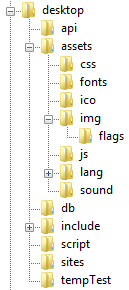
\includegraphics[width=0.25\textwidth]{images/folderStructure.png}
        \caption{The Code Folder Structure}
        \label{fig:folderStructure}
\end{figure}

\noindent{\textbf{web:} This is the main directory for the web interface.}\\
\\
\textbf{backend:} This is the main directory for the back end of the system.\\
\\
\textbf{api:} Is intended to contain API which are not JavaScript or PHP code.\\
\\
\textbf{assets:} Contains every asset in the system. Images, JavaScript, sound, fonts, CSS and language files.\\
\\
\textbf{assets - css:} Contains the CSS files for the system.\\
\\
\textbf{assets - fonts:} Contains special fonts for the system.\\
\\
\textbf{assets - ico:} Contains the icon files for the system.\\
\\
\textbf{assets - img:} Contains the static image resources for the system.\\
\\
\textbf{assets - img - flags:} Contains images of flags, used for changing language.\\
\\
\textbf{assets - js:} Contains all JavaScript in the system, files are named as they fit to PHP files, as far as this is possible.\\
\\
\textbf{assets - lang:} Contains all language files to the system. Each webpage and some JavaScripts, have their own language sub-folder .\\
\\
\textbf{db:} Contains the database files. All active database functions are stored in the file ``db.php''\\
\\
\textbf{include:} Contains any JavaScript or PHP code that is not developed by this project, but that is included in the system.\\
\\
\textbf{script:} Contains PHP scripts which do not display anything, but rather work to execute some functions.\\
\\
\textbf{sites:} Contains .html and .php files which correspond to a webpage on the web interface.\\
\\
\textbf{tempTest:} A folder for any need of generating files during development.

 - old
	\chapter{Problem Statement}
As the previous chapter explained, children's increase in media usage is becoming a problem. This is a problem we want to solve by the usage of modern technology, internet applications and physical recognition of users.\\
In this chapter a formal definition of the problem is written together with an emphasis on what challenges this problem rises.\\


\begin{verse}
\textit{Parents are not able to help their children administer their IT/TV consumption.\\
This results in their children getting a lessened learning ability, a bad sleeping pattern and a higher risk of type 2 diabetes.\\
How can hardware identification and webservices give parents the tools to help their children manage their media consumption?}\\
To address this problem, we face the following technical challenges:
	\begin{itemize}
		\item How do we identify unique users in a subtle and child friendly way.
		\item How do we enforce restrictions on media devices.
		\item How do we facilitate concepts as rules, permissions and chores without parents interaction.
	\end{itemize}
\end{verse}


With this formal statement of the problem in mind, the next chapter goes into detail of how we intend to solve these challenges.

%English: Parents are not able of helping their children administer their IT/TV consumption.
%This results in their kids getting a lessened learning ability, a bad sleeping pattern and more.
%How can smart home technology give parents the tools they need to help their children administer their IT/TV consumption?

%Edited version:
%How can hardware identification and webservices give parents the tools to help their children manage their media consumption. 
%(Childrens media consumptions is increasing, giving higher risks of type 2 diabetes.
	
	
	% Part Solution
	\part{Solution}
	\chapter{Overall System Design}
In this chapter we present the overall design of Media-Online Management(MOM). First we will present how we intend the users to use MOM. Then general concepts will be introduced which is an essential part of the system and will be mentioned several times hereafter. Thirdly the requirements of MOM will be explained in more detail. Finally the system architecture will be presented.    


\section{Media-Online Management} %name our system: temp name: Media-Online Management or MOM
The Media-Online Management (MOM) is the system that is our solution on the problem statement. To give an overview of the complete system a rich picture \citep{OOAD} have been made, see the figure \ref{fig:systemoverview}. The figure shows a home environment with a TV (media), computer and an internet connection, and it shows a server. 

There are two main use patterns. The first is a parent who manage their MOM using the website from the PC to add, change or delete system settings. This is pictured in the bottom left-side corner in figure \ref{fig:systemoverview}. 

The second use pattern is pictured in the upper left corner of the figure. It is a child user who wants to use a media which in this case is the television. But to watch television it need power and its power source is blocked by the controller. So the child needs to scan his tag and then the controller sends a message to the server which then reply whether the television can be turned on or not. When the child is done he must scan again such that points can be withdrawn from his user profile. If the child does not have any points he cannot turn on the television nor can he turn it on if a rule or permission does not allow it. If a parent wants to watch television without being restricted in any way he can make a rule that gives him unlimited access, but he would still need to scan his tag before and after using the television. \fixme{Vil vi lave en lille evaluering om vi synes det er fair at forældrene også skal scanne?}

\begin{figure}
	\centering
		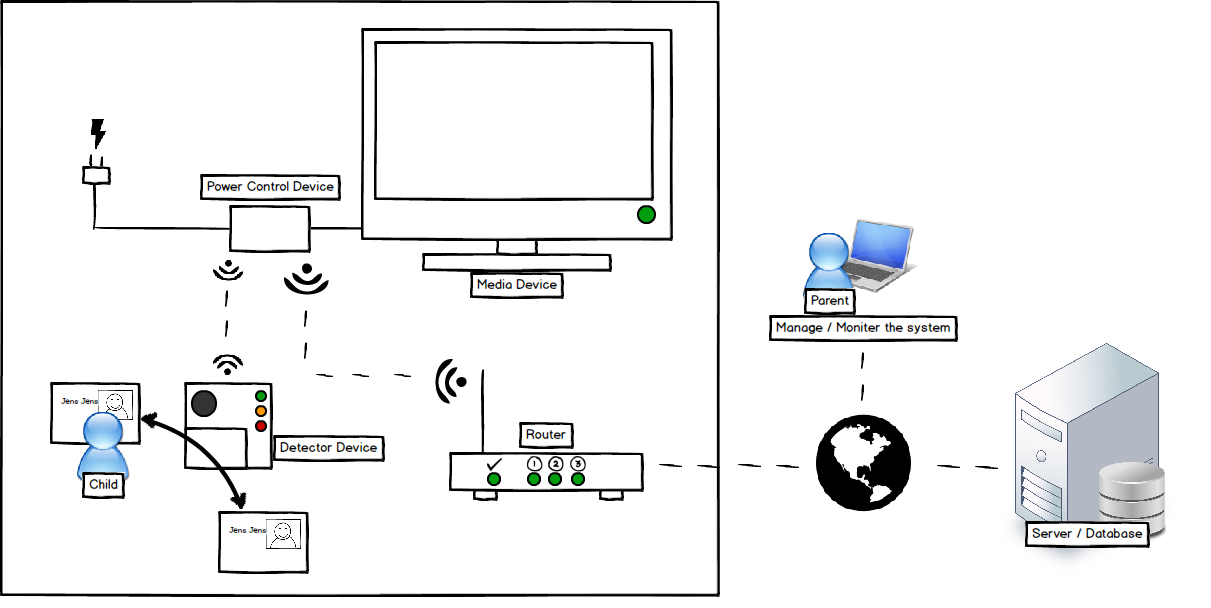
\includegraphics[width=1.00\textwidth]{images/systemoverview2.png}
	\caption{system overview}
	\label{fig:systemoverview}
\end{figure}

On the server there will be a database, files that generate the website, a web service, and a daemon. These elements of the system will be explained further in section \vref{sec:RequirMOM} and after that the system architecture can be presented in section \vref{sec:sysArchitecture}. However, we need to explain some of the concepts that will be used in connection with this system.

\chapter{General Design Concepts}
\label{chapter:concepts}
%Go into detail about rules, permission, chores
In the Media-Online Management there are a few concepts that will be used through out the report. These are chore, permission and rules. The meaning of each will be explain in the following sections.

\section{Chore}
A chore in MOM is a representation of a house chore that is to be done regularly. We have included chore into this system to encourage children to help with the house chores which gives more time for media as a reward. Therefore each chore needs a number of points which will be given when the child has done the house chore. 
An example on a house chore could be to take out the garbage, then the chore in MOM would have a name: 'take out garbage', possible a bigger description of the chore: 'remember to sort the garbage into the correct trash cans' and when the chore is done some points is given: '10'.  

One disadvantage about the chore design is that the parent needs to use the website to award the child with points for doing a chore. We would have liked to automate it further, but to limit the scope of the project this would be future work.  
  
%is a subtype of rules. But we like to differentiate on rules not being necessary for the usage of the system, where permissions is. Permissions is only used to tell the system the normal allowed usage of media and rules is there to overwrite these permissions in special cases, or if the user wants to customize the system.\\



\section{Rule}
\label{sec:rule}
In the system a rule can be many things the following is just a few examples of rules:

\begin{itemize}
	\item Susan has access to use the PC from 15:00 to 17:00 each day.
	\item The first Monday in a month Peter's points is increased by 100
	\item Mom and Dad's profiles have unlimited time and unrestricted access to any media
\end{itemize}

The rule has been included because it gives the parents a more powerful method to control their children's use of medias. 
But there is one disadvantage with rules, it might be complicated for the user to understand how to use them. 
This means we must take care to design the concept of rules, so that it is easy to use and understand their effects.

A rule should be connected to one or more user profiles since the rules otherwise would be unnecessary. A rule consist of a name, a set of actions and  a restricted set of conditions depending on the actions. A condition is used to decide when a rule is relevant which is when all conditions fits. An action is something that can or should be done if all of the rule's conditions hold.
To see a quick overview of the different conditions and their name:

\begin{description}
	\item[Timeperiod] the action can be done in this time period.% \fixme{Does this still exist?} yes
	\item[Controller on] the action can be done if a specific controller is turn on. 
	\item[Controller off] the action can be done if a specific controller is turn off. 
	\item[True] The action can always be taken. This is actually kind of a time period but there is no time bounds.
\end{description}

An overview of the actions and their name is listed below:

\begin{description}
	\item[Block user] it will block the profiles of all profiles connected to the rule. 
	\item[Add points] it will add points to the profiles' points.
	\item[Delete points]  it will delete points to the profiles' points.  
	\item[Set maximum of point] it will set a maximum number of points that a profile can have. 
	\item[Unlimited time] it will give the profile unlimited time to be spend on any media. 
	\item[Access any controller] it will give the profile access to any media in the system. 
	\item[Cannot access any controller] the profile will not have access to any media. 
	\item[Access controller] it will give the profile access to a specific media. 
	\item[Cannot access controller] it will block the user from using a specific media. 
\end{description}

Two designs have been made over rule. The first design is explained in the appendix \vref{appendixFirstRuleDesign}. The final design is of the rule is explained later in this section. The main difference is that in the first design is an extra type of condition timestamp. But late into the implementation of MOM we found that it would not be needed and therefor reworked the design, into what follows.\\
\\
The rule's structure is presented in a grammar in listing	\ref{grammar2} expressed in Extended Backus-Naur Form(EBNF) \citep{CoPL}.
A nonterminal is en-captured in $<>$ and a terminal is just a word or en-captured in "". 
Also the grouping is used represented in $()$, the replica symbol is $*$, comments is $(**)$ and alternative is $|$. 

A rule consist of a name and one of five action and condition sets which determine which actions and conditions can be combined. A rule can have several actions and conditions but only from the same set, see line 1-7. The action set is presented from 9-23 where all has a specific name, some have a specific Controller represented as a number and some has points which is a number. The condition set likewise represented from 9-23 and the condition types are presented from 25-30. There are three types but they each have a specific name. One type has a Controller, another only the name 'True' and the last has a timeperiod. The timeperiod has two timestamps and if it is repeatable it has a string representation of the weekdays and a representation of how it is repeatable. 

\begin{lstlisting}[label=grammar2, caption=Grammar of a rule in EBNF]
<Rule>:= <name> (
	 	  (<ActionsetSet1><ConditionSet1>)*
		| (<ActionsetSet2><ConditionSet2>)*
		| (<ActionsetSet3><ConditionSet3>)*
		| (<ActionsetSet4><ConditionSet4>)*
		| (<ActionsetSet5><ConditionSet5>)*
	)

<ActionsetSet1> := "Block user" 
<ConditionSet1> := <ConditionTimeperiod> |<ConditionTrue>

<ActionsetSet2> := ("Add points" | "Delete points") <Points>
<ConditionSet2> := <ConditionTimeperiod>

<ActionsetSet3> := "Set maximum of point" <Points>
<ConditionSet3> := <ConditionTrue>

<ActionsetSet4> := "Unlimited time" | ("Access any controller" | "Cannot access any controller") <Controller>
<ConditionSet4> := <ConditionTimeperiod> | <ConditionTrue> 

<ActionsetSet5> := ("Access controller" | "Cannot access controller")<Controller>
<ConditionSet5> :=	<ConditionTimeperiod> |	<ConditionTrue>	|	<ConditionElse>	
				
<ConditionTimeperiod> :=  "TimePeriod" <Timestamp> <Timestamp> <Repeatable>					
<Repeatable> :=   <Weekdays> <Repeat> | Nill

<ConditionTrue> := "True" 
<ConditionElse>:= ("Device on" | "Device off") <Controller>
				
<Name> := ALPHA*  (* Upper and lowercase ASCII letters (A-Z,a-z) *)
<Controller> := DIGIT* (* Decimal digits (0-9) *)
<Points> := DIGIT*
<Timestamp> := 4*DIGIT,"-",2*DIGIT,"-",2*DIGIT, " ",2*DIGIT,":"2*DIGIT,":"2*DIGIT  (*YYYY-MM-DD HH:mm:ss*)
<Weekdays> := ("monday"| "tuesday"| "wednesday"| "thursday"| "friday"| "saturday"| "sunday")*
<Repeat> := "weekly" | "biweekly" | "triweekly" | "first in month" | "last in month"
\end{lstlisting}
		
\subsection{Examples of Rules}
In this section some examples of rules for a profile will be given.

The first example could be that the profile Peter gets point for each football training and the football training is Monday and Thursday from 18:00 to 19:30 each week. Then the action could be add 25 points to Peter when condition holds. The condition is from 19:30 to 19:30 where the day is 'Monday, Thursday' and it is repeated weekly. \\

The second example could be that Susan is grounded from the 2nd December to the 6th December both at 6 p.m.. In the system there will be a condition with a Timeperiod which is 2nd December 2013 18:00 to 6th December 18:00.
and an action that is 'Block user' such that she cannot use any media or gain points in this period. \\

If the parents should make a rule which give themselves unlimited time and access to any media. The condition would be True and the actions would be 'Unlimited time' and 'Access any controller'.\\\\  


\section{Permission}
Permission in this system is whether a user have access to a given media. Permissions can also be expressed as a rule, but it is easier to make and understand a permission. This is also the main reason for differentiating the two for the user. 

A permission need a user and a controller. When a user then is connected to a permission it means this user has permission to use the media which is connected to this controller. An example could be that Peter has permission to use the TV. 

A permission is different from a rule in two ways according to the data structure. First, a permission does not need a condition, it is always true. Secondly a permission is always of the action type ''Access Controller''.\\
This means that permissions is only an abstraction making an easier understanding for the user.


\section{Permission and Rules Precedence}
It should be possible to override permissions and rules with another rule, but then some priority rules  need to be established. 
For the overriding of the two to be relevant they need to overlap in time which mean that the condition should use Timeperiod or True. Also if it is a rule then it should have an action with the name 'Cannot access controller', 'Access controller', 'Cannot access any controller' or 'Access any controller' to be relevant. So from the grammar \ref{grammar2} it is the rule sets $<name> <ActionsetSet4><ConditionSet4>$  and $<name> <ActionsetSet5><ConditionSet5>$ that need the priority.

We came to the conclusion that rules always have precedence over permissions. But if the conflict is among two rules it is a more complex set of precedence rules. First to determine the precedence we look at the action's name. See figure \ref{fig:precendence} where the precedence graph is shown. Notice that the precedence for 'Cannot access controller' and 'Access controller' can be either way depending on the condition. Otherwise both of them has priority over 'Access any controller' which also has priority over 'Cannot access any controller'. 
  
\begin{figure}
	\centering
		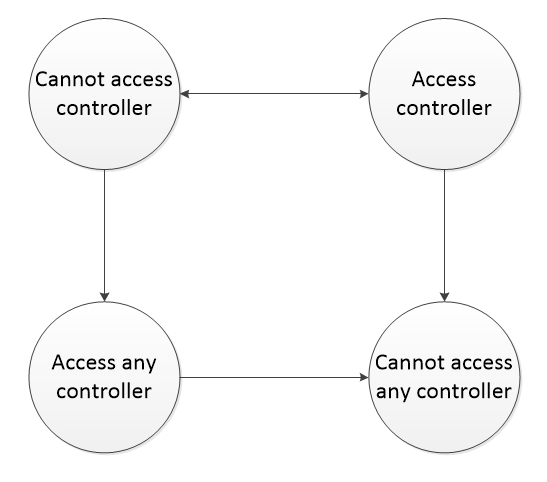
\includegraphics[width=0.75\textwidth]{images/precendence.jpg}
	\caption{Precedence of rules}
	\label{fig:precendence}
\end{figure}

When the condition determines the precedence we have different combinations:

\begin{itemize}
	\item If one is True and the other is Timeperiod then the rule with the Timeperiod has the higher precedence
	\item If both is True then Access controller has the precedence.
	\item If both is Timeperiod:
		\begin{itemize}
			\item If both is repeatable or non-repeatable%\fixme{First time we talk about non-repeatable} - not really look in grammar and text above, just saying if it is repeateble 
			then Access controller has the precedence
			\item If one is repeatable and the other is nonrepeatable then the rule with the nonrepeatable Timeperiod has the higher precedence.
		\end{itemize}
\end{itemize}

These precedence rules do not avoid all possible conflict but it limits them.  


This conclude the general concepts that will be used through out the remainder of the report. Next further details about the requirements of MOM is described.


\section{Requirements of MOM}
\label{sec:RequirMOM}

In the analysis we came to the conclusion that the following items is necessary for MOM: 
\begin{itemize}
	\item A device to toggle the power of an electronic media
	\item An individual key for each child that can be read by the device
	\item A website to set up rules, permissions and view/modify allowed usage of electronic media
\end{itemize} 


The first item is called controller in this system, the second is the tag and the last is the website on the computer. But also new components of the system is necessary. As explained in the previous section a daemon is needed to check the relevant rules and perform the appropriate actions if the conditions holds. Also during the following sections we find that a web service is needed. 

In the following sections the specification of the website, controller and tag, web service and daemon will be explained, before the design and implementation will be presented for each of them in the following chapters.  

\subsection{MOM's Website}
\label{subsection:momswebsite}
A Media-Online Management (MOM) owner needs a way to manage the system and for this a website will be made. There are several requirements for this website:

\begin{itemize}
	\item Register a new MOM together with a user profile which is a manager of this system
	\item Make it possible to add, edit and delete user profiles in an existing MOM 
	\item Make it possible to add, edit and delete Controllers from an existing MOM
	\item There should be a way to add, edit and delete Tags to the system. Also a tag should be connected to a user profile
	\item There need to be an option to add, edit and delete rules, permissions and chores from a system
	\item The user should be able to connect rules and permission with one or more user profiles. The connection should also be able to be removed without removing the rule or permission
	\item When a chore is done in the real world by a child profile then by connecting this profile to a chore, points should be added to his profile
\end{itemize}

There are also some requirements that is nice for the parents to use, but they are not essential for MOM system:

\begin{itemize}
	\item present the media consumption data as graphs or logs such that the parents easy can get an overview of their children's media consumption 
	\item present data from MOM in a calendar that shows rule and permission with profiles for whom this is relevant. The calendar should also show when a chore have been done and by who.
\end{itemize}

In chapter \fixme{insert ref} the design and implementation of the website will be presented in more detail. 
 

\subsection{Tag and Controller}
The tag used in this system is using Radio-frequency Identification (RFID). The tag need to be uniquely identified in MOM and it must uniquely identify its user. The tag is used in combination with the controller.

The controller is an Arduino which is connected to a tag reader. Like the tag it need to be uniquely identified in MOM. The controller must be able to do the following.

\begin{itemize}
	\item Read the data from the tag
	\item Send and receive messages from the server
	\item Control the power source of the media 
	\item Temporarily store the tag id that activated this controller
	\item Keep track of the time spent between activation of the media to its end
\end{itemize}
 
The design and implementation of the controller will be explained further in chapter \fixme{insert chapter ref}. 

The controller must communicate with the server and this is done via a web service.

\subsection{The web service}

The web service is used to parse the relevant data to the controller. Its requirements are:

\begin{itemize}
	\item Receive and send messages to the controller
	\item From a tag and controller it should be able to determine whether a user may use the media which is connected to the controller
	\item It must be able to subtract points from a user after he has been using a media
	\item It should able to calculate when a controller should be turned off because of a rule, permission or point.
\end{itemize}

The web service's design and implementation is explained further in chapter \fixme{ref to chapter}.


\subsection{Daemon}
The daemon is used to update data in the database from a rule which the user have made at some point. The daemon does not have any direct contact to a client. The daemon should handle any rule that is time determined so the condition is either Timestamp or Timeperiod. Then the daemon should do the appropriate action which could be add points to user or block a user.

The design and implementation of the daemon is presented in detail in chapter \fixme{ref to chapter}. 
 
\section{System Architecture}
\label{sec:sysArchitecture}
Now that all subsystem of the Media-Online Management have been presented the overall system architecture can be explained. MOM is using the client server architecture which is shown in the figure \ref{fig:serveroverview} \citep{OOAD}. This system has two types of client the first is a controller and the second is a computer where the user manages the system via the web site. The controller is depended on the web service on the server and the computer is depended on the web site. On the server there is the web site, web service and daemon which all are depended on the functions component, MySQLHelper class and data component. In the function component there are several functions to work on the data in the database and this component is depended on MySQLHelper because it should establish the database connection and parse the quires on to the database. 

\begin{figure}
	\centering
		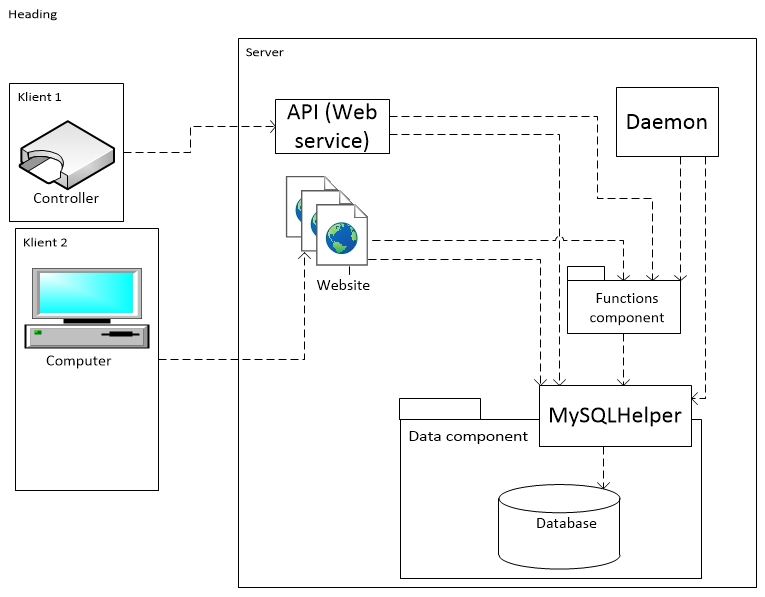
\includegraphics[width=1.25\textwidth,  angle=90]{images/serveroverview.jpg}
	\caption{system architecture}
	\label{fig:serveroverview}
\end{figure}

In the following chapters design and implementation of the web site, web service, deamon and database will be presented.

 



	\chapter{Hardware}
\label{chap:hardware}
In this section the hardware choices of this project will be talked about and analyzed. First the choice of hardware platform will be discussed, next the choice of hardware identification needed for the system and then the server setup. Followed each by a conclusion stating the chosen option.

\section{Hardware Platform}
\label{HardwarePlatform}
In order to control the power to a media(i.e. Television or Computer), some analog power control is needed. This can be controlled by an embedded microcontroller, the choice of hardware platform is, in our case, to pick the best microcontroller for the project. A development board is usually used during development . A development board is a single printed circuit board with a microcontroller and everything needed to get the microcontroller running. Every I/O\footnote{Input/Output}(generally General-purpose I/O) of the microcontroller is also made easily available using group pins. Picking a hardware platform is then condensed into picking a development board. Following is a comparison of a few different development boards.

\subsubsection{Arduino}
Arduino development boards come in a few variations, but common among all but one of them is that they are based on Atmel microcontrollers. Along with the development boards, Arduino also comes with its own software library \texttt{Wiring} which simplifies common I/O tasks. The Arduino development boards also implement a standard called \texttt{shields}, which are expansion circuit boards with pin headers that fit onto the development boards, with additional pins so that shields can be stacked. This makes the hardware platform easily extendable and flexible using this stacking system. Examples of shields could be GPS, Ethernet, LCD displays or breadboards.\citep{arduinoCC}


\subsubsection{Teensy}
Teensy, like Arduino is based on a Atmel microcontroller, but unlike Arduino is made to be as small as possible. Teensy also supplies an add-on library that makes Arduino programs compatible. Power is supplied via USB instead of a dedicated power input on the Arduino, which makes it cheaper. Teensy does not have an equivalent of shields.\citep{teensyPJRC}


\subsubsection{Raspberry Pi}
Raspberry Pi, unlike Arduino and Teensy, uses a ``full-sized'' ARM processor, which makes it more like a regular computer than a microcontroller. Despite that it has GPI/O pins just like Arduino and Teensy, which means that it has the capabilities needed for the project. Being ARM based means that the Raspberry Pi can also install operating systems such as Linux based operating systems. The ARM processor is also many times more powerful than the Atmel microcontrollers. This however comes with negatives such as higher power consumption, unused modules(GPU, sound or SD card storage) resulting in a larger board and a higher cost. \citep{raspberrypi}

\subsection{Conclusion - Platform}
In conclusion the platform chosen is Arduino. Arduino is chosen because of their shield design, which enables the use of a Ethernet shield as well as a RFID shield. Some of the group members has also already worked with Arduino, which means a lower learning curve.

\section{Hardware Identification}
In order for the person using the system to identify themselves, there has to be some form of hardware identification. This hardware identification has to be unique for that person, so that the system can calculate the allowed time the user can use on that media. Several factors have to be considered when choosing what hardware identification method to use, such as cost, user friendliness and security. Following is a comparison between some of the hardware identification methods available.

\subsubsection{RFID}
\label{rfidsect}
RFID, short for Radio-frequency Identification, is a method of using either passive or active tags for transferring data between a reader and a tag. A tag is an embedded chip with an antenna, that when receiving power transmits the data on the chip to any readers within range. Active tags have their own power source and thus can be scaled to emit their data over long distances. Passive tags on the other hand do not have an internal power source, and instead is powered by the reader via magnetic fields. This makes passive tags work on smaller ranges.\citep{rfidAndNfc} A tag can be compared to a bar code, with the difference being that tags scale much better when needing more data storage and the tag does not have to be visible, i.e. it can be embedded into for example key-cards, jewelry and such.

\subsubsection{NFC}
NFC, short for Near Field Communication, is a set of standards for the same technology that RFID uses. The differences between them is that NFC is a strict standard, uses only passive tags and only works over small distances.\citep{rfidAndNfc} NFC is also the technology being embedded in smartphones, which means that the projects system could be made compatible with apps.\\
\\
Fingerprints and iris recognition was also considered, but dismissed these solutions based on pricing and the fact that the human body changes a lot during the first 20 years of life.\citep{irisid}

\subsection{Conclusion - Identification}
In conclusion the identification chosen is RFID, because it could be provided by the university, however, originally NFC was preferred. 
The RFID has been chosen because it is easily accessible, and all of the practices used with RFID can be used with NFC. The reason for choosing NFC over RFID, is that it is a well defined standard, it is compatible with the technology used in smartphones and it is short range so no accidental reads happen. The reason for choosing NFC/RFID over fingerprint is that the security needed for fingerprints do not scale with simplicity and the possibility of a child's fingerprint changing too much. The reason for choosing NFC/RFID over iris is primarily the cost, as the cost of a high quality camera is too high since multiple cameras would be needed.

\section{Servers}
In order to maintain the wast amount of information collected from the users and in order to offer a graphical interface to add rules, permissions and chores to the system a server setup is needed.\\
Such server work can be done from a private home or centralized global server, maintained by the manufacturer of the system.\\

Listed here is the pros and cons of having a decentralized server setup versus centralized server setup.\fixme{kilde}\\

\textbf{Decentralized Server Setup}\\
Pros:
\begin{itemize}
	\item Maintains proper functionality even if the internet connection out of the house is broken.
	\item Could be integrated in a Smart Home setup
\end{itemize}

Cons:
\begin{itemize}
	\item Each user will have to setup the system themselves or pay for a professional
  \item If the server malfunctions the user is the one with the problem
  \item Need to own a domain name and an external IP address in order to access the system from outside
\end{itemize}

\textbf{Centralized Server Setup}\\
Pros:
\begin{itemize}
	\item The setup of the system is for the user only registering on the website
	\item The user does not have to pay for extra electricity consumption of the server
	\item If the server fails, proper security measures can be setup to handle these problems
\end{itemize}

Cons:
\begin{itemize}
	\item If the internet connection malfunctions for what ever reason, the system will not work optimally.
  \item The user is limited to the functionality that is offered
\end{itemize}

As can be seen in the lists, most pros in the central setup is cons in the decentralized setup and vice verse.\\
This project focuses on developing a user friendly and upgradeable system, and therefore a centralized server setup has been chosen. The centralized system offers the easiest way for users to get started and it also makes it easier to deal with problems. The only problem that a user can face, is the lack of internet connection or power, which in our modern time is unlikely for a considerable amount of time.\\
Also the user would never have to do anything to keep their system up to date, since this would be handled on the server side.

	\chapter{General Design Concepts}
\label{chapter:concepts}
%Go into detail about rules, permission, chores
In the Media-Online Management there are a few concepts that will be used through out the report. These are chore, permission and rules. The meaning of each will be explain in the following sections.

\section{Chore}
A chore in MOM is a representation of a house chore that is to be done regularly. We have included chore into this system to encourage children to help with the house chores which gives more time for media as a reward. Therefore each chore needs a number of points which will be given when the child has done the house chore. 
An example on a house chore could be to take out the garbage, then the chore in MOM would have a name: 'take out garbage', possible a bigger description of the chore: 'remember to sort the garbage into the correct trash cans' and when the chore is done some points is given: '10'.  

One disadvantage about the chore design is that the parent needs to use the website to award the child with points for doing a chore. We would have liked to automate it further, but to limit the scope of the project this would be future work.  
  
%is a subtype of rules. But we like to differentiate on rules not being necessary for the usage of the system, where permissions is. Permissions is only used to tell the system the normal allowed usage of media and rules is there to overwrite these permissions in special cases, or if the user wants to customize the system.\\



\section{Rule}
\label{sec:rule}
In the system a rule can be many things the following is just a few examples of rules:

\begin{itemize}
	\item Susan has access to use the PC from 15:00 to 17:00 each day.
	\item The first Monday in a month Peter's points is increased by 100
	\item Mom and Dad's profiles have unlimited time and unrestricted access to any media
\end{itemize}

The rule has been included because it gives the parents a more powerful method to control their children's use of medias. 
But there is one disadvantage with rules, it might be complicated for the user to understand how to use them. 
This means we must take care to design the concept of rules, so that it is easy to use and understand their effects.

A rule should be connected to one or more user profiles since the rules otherwise would be unnecessary. A rule consist of a name, a set of actions and  a restricted set of conditions depending on the actions. A condition is used to decide when a rule is relevant which is when all conditions fits. An action is something that can or should be done if all of the rule's conditions hold.
To see a quick overview of the different conditions and their name:

\begin{description}
	\item[Timeperiod] the action can be done in this time period.% \fixme{Does this still exist?} yes
	\item[Controller on] the action can be done if a specific controller is turn on. 
	\item[Controller off] the action can be done if a specific controller is turn off. 
	\item[True] The action can always be taken. This is actually kind of a time period but there is no time bounds.
\end{description}

An overview of the actions and their name is listed below:

\begin{description}
	\item[Block user] it will block the profiles of all profiles connected to the rule. 
	\item[Add points] it will add points to the profiles' points.
	\item[Delete points]  it will delete points to the profiles' points.  
	\item[Set maximum of point] it will set a maximum number of points that a profile can have. 
	\item[Unlimited time] it will give the profile unlimited time to be spend on any media. 
	\item[Access any controller] it will give the profile access to any media in the system. 
	\item[Cannot access any controller] the profile will not have access to any media. 
	\item[Access controller] it will give the profile access to a specific media. 
	\item[Cannot access controller] it will block the user from using a specific media. 
\end{description}

Two designs have been made over rule. The first design is explained in the appendix \vref{appendixFirstRuleDesign}. The final design is of the rule is explained later in this section. The main difference is that in the first design is an extra type of condition timestamp. But late into the implementation of MOM we found that it would not be needed and therefor reworked the design, into what follows.\\
\\
The rule's structure is presented in a grammar in listing	\ref{grammar2} expressed in Extended Backus-Naur Form(EBNF) \citep{CoPL}.
A nonterminal is en-captured in $<>$ and a terminal is just a word or en-captured in "". 
Also the grouping is used represented in $()$, the replica symbol is $*$, comments is $(**)$ and alternative is $|$. 

A rule consist of a name and one of five action and condition sets which determine which actions and conditions can be combined. A rule can have several actions and conditions but only from the same set, see line 1-7. The action set is presented from 9-23 where all has a specific name, some have a specific Controller represented as a number and some has points which is a number. The condition set likewise represented from 9-23 and the condition types are presented from 25-30. There are three types but they each have a specific name. One type has a Controller, another only the name 'True' and the last has a timeperiod. The timeperiod has two timestamps and if it is repeatable it has a string representation of the weekdays and a representation of how it is repeatable. 

\begin{lstlisting}[label=grammar2, caption=Grammar of a rule in EBNF]
<Rule>:= <name> (
	 	  (<ActionsetSet1><ConditionSet1>)*
		| (<ActionsetSet2><ConditionSet2>)*
		| (<ActionsetSet3><ConditionSet3>)*
		| (<ActionsetSet4><ConditionSet4>)*
		| (<ActionsetSet5><ConditionSet5>)*
	)

<ActionsetSet1> := "Block user" 
<ConditionSet1> := <ConditionTimeperiod> |<ConditionTrue>

<ActionsetSet2> := ("Add points" | "Delete points") <Points>
<ConditionSet2> := <ConditionTimeperiod>

<ActionsetSet3> := "Set maximum of point" <Points>
<ConditionSet3> := <ConditionTrue>

<ActionsetSet4> := "Unlimited time" | ("Access any controller" | "Cannot access any controller") <Controller>
<ConditionSet4> := <ConditionTimeperiod> | <ConditionTrue> 

<ActionsetSet5> := ("Access controller" | "Cannot access controller")<Controller>
<ConditionSet5> :=	<ConditionTimeperiod> |	<ConditionTrue>	|	<ConditionElse>	
				
<ConditionTimeperiod> :=  "TimePeriod" <Timestamp> <Timestamp> <Repeatable>					
<Repeatable> :=   <Weekdays> <Repeat> | Nill

<ConditionTrue> := "True" 
<ConditionElse>:= ("Device on" | "Device off") <Controller>
				
<Name> := ALPHA*  (* Upper and lowercase ASCII letters (A-Z,a-z) *)
<Controller> := DIGIT* (* Decimal digits (0-9) *)
<Points> := DIGIT*
<Timestamp> := 4*DIGIT,"-",2*DIGIT,"-",2*DIGIT, " ",2*DIGIT,":"2*DIGIT,":"2*DIGIT  (*YYYY-MM-DD HH:mm:ss*)
<Weekdays> := ("monday"| "tuesday"| "wednesday"| "thursday"| "friday"| "saturday"| "sunday")*
<Repeat> := "weekly" | "biweekly" | "triweekly" | "first in month" | "last in month"
\end{lstlisting}
		
\subsection{Examples of Rules}
In this section some examples of rules for a profile will be given.

The first example could be that the profile Peter gets point for each football training and the football training is Monday and Thursday from 18:00 to 19:30 each week. Then the action could be add 25 points to Peter when condition holds. The condition is from 19:30 to 19:30 where the day is 'Monday, Thursday' and it is repeated weekly. \\

The second example could be that Susan is grounded from the 2nd December to the 6th December both at 6 p.m.. In the system there will be a condition with a Timeperiod which is 2nd December 2013 18:00 to 6th December 18:00.
and an action that is 'Block user' such that she cannot use any media or gain points in this period. \\

If the parents should make a rule which give themselves unlimited time and access to any media. The condition would be True and the actions would be 'Unlimited time' and 'Access any controller'.\\\\  


\section{Permission}
Permission in this system is whether a user have access to a given media. Permissions can also be expressed as a rule, but it is easier to make and understand a permission. This is also the main reason for differentiating the two for the user. 

A permission need a user and a controller. When a user then is connected to a permission it means this user has permission to use the media which is connected to this controller. An example could be that Peter has permission to use the TV. 

A permission is different from a rule in two ways according to the data structure. First, a permission does not need a condition, it is always true. Secondly a permission is always of the action type ''Access Controller''.\\
This means that permissions is only an abstraction making an easier understanding for the user.


\section{Permission and Rules Precedence}
It should be possible to override permissions and rules with another rule, but then some priority rules  need to be established. 
For the overriding of the two to be relevant they need to overlap in time which mean that the condition should use Timeperiod or True. Also if it is a rule then it should have an action with the name 'Cannot access controller', 'Access controller', 'Cannot access any controller' or 'Access any controller' to be relevant. So from the grammar \ref{grammar2} it is the rule sets $<name> <ActionsetSet4><ConditionSet4>$  and $<name> <ActionsetSet5><ConditionSet5>$ that need the priority.

We came to the conclusion that rules always have precedence over permissions. But if the conflict is among two rules it is a more complex set of precedence rules. First to determine the precedence we look at the action's name. See figure \ref{fig:precendence} where the precedence graph is shown. Notice that the precedence for 'Cannot access controller' and 'Access controller' can be either way depending on the condition. Otherwise both of them has priority over 'Access any controller' which also has priority over 'Cannot access any controller'. 
  
\begin{figure}
	\centering
		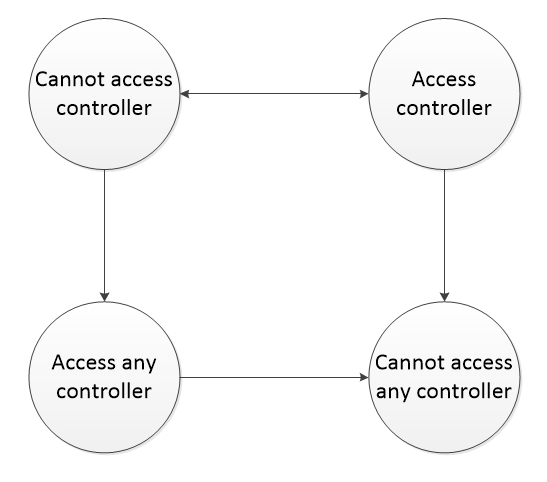
\includegraphics[width=0.75\textwidth]{images/precendence.jpg}
	\caption{Precedence of rules}
	\label{fig:precendence}
\end{figure}

When the condition determines the precedence we have different combinations:

\begin{itemize}
	\item If one is True and the other is Timeperiod then the rule with the Timeperiod has the higher precedence
	\item If both is True then Access controller has the precedence.
	\item If both is Timeperiod:
		\begin{itemize}
			\item If both is repeatable or non-repeatable%\fixme{First time we talk about non-repeatable} - not really look in grammar and text above, just saying if it is repeateble 
			then Access controller has the precedence
			\item If one is repeatable and the other is nonrepeatable then the rule with the nonrepeatable Timeperiod has the higher precedence.
		\end{itemize}
\end{itemize}

These precedence rules do not avoid all possible conflict but it limits them.  


This conclude the general concepts that will be used through out the remainder of the report. Next further details about the requirements of MOM is described.
	\chapter{Requirements of MOM}
\label{chap:RequirMOM}

In the analysis we came to the conclusion that the following items is necessary for MOM: 
\begin{itemize}
	\item A device to toggle the power of an electronic media
	\item An individual key for each child that can be read by the device
	\item A website to set up rules, permissions and view/modify allowed usage of electronic media
\end{itemize} 


The first item is called controller in this system, the second is the tag and the last is the website on the computer. But also new components of the system is necessary. 
As the expanding of the rule concept went on, it became apparent that some of the rules needed to be handled autocratically when the conditions held. For this a daemon can be used, and in our case it was.\\
\\
Also during the following sections we find that a web service is needed. 

In the following sections the specification of the website, controller and tag, web service and daemon will be explained, before the design and implementation will be presented for each of them in the following chapters.  

\section{MOM's Website}
\label{section:momswebsite}
A Media-Online Management (MOM) owner needs a way to manage the system and for this a website will be made. There are several requirements for this website:

\begin{itemize}
	\item Register a new MOM together with a user profile which is a manager of this system\fixme{Not for the user}
	\item Make it possible to add, edit and delete user profiles in an existing MOM 
	\item Make it possible to add, edit and delete Controllers from an existing MOM
	\item There should be a way to add, edit and delete Tags to the system. Also a tag should be connected to a user profile
	\item There need to be an option to add, edit and delete rules, permissions and chores from a system
	\item The user should be able to connect rules and permission with one or more user profiles. The connection should also be able to be removed without removing the rule or permission
	\item When a chore is done in the real world by a child profile then by connecting this profile to a chore, points should be added to his profile
\end{itemize}

There are also some requirements that is nice for the parents to use, but they are not essential for the MOM system:

\begin{itemize}
	\item present the media consumption data as graphs or logs such that the parents easy can get an overview of their children's media consumption 
	\item present data from MOM in a calendar that shows rule and permission with profiles for whom this is relevant. The calendar should also show when a chore have been done and by who.
\end{itemize}

In chapter \vref{chap:website} the design and implementation of the website will be presented in more detail. 
 

\section{Tag and Controller}
The tag used in this system is using Radio-frequency Identification (RFID). The tag need to be uniquely identified in MOM and it must uniquely identify its user. The tag is used in combination with the controller.

The controller is an Arduino which is connected to an RFID reader. Like the tag it need to be uniquely identified in MOM. The controller must be able to do the following.

\begin{itemize}
	\item Read the data from the tag
	\item Send and receive messages from the server
	\item Control the power source of the media 
	\item Temporarily store the tag id that activated this controller
	\item Keep track of the time spent between activation of the media to its end
\end{itemize}
 
The design and implementation of the controller will be explained further in chapter \vref{chap:controller}. 

The controller must communicate with the server and this is done via a web service.

\section{API}

The API is used to parse the relevant data to the controller. Its requirements are:

\begin{itemize}
	\item Receive and send messages to the controller
	\item From a tag and controller it should be able to determine whether a user may use the media which is connected to the controller
	\item It must be able to subtract points from a user after he has been using a media
	\item It should be able to calculate when a controller should be turned off because of a rule, permission or point.
\end{itemize}

The web service's design and implementation is explained further in chapter \vref{chap:api}.


\section{Daemon}
The daemon is used to update data in the database from a rule which the user have made at some point. The daemon does not have any direct contact to a client. The daemon should handle any rule that is time determined so the condition is a Timeperiod. Then the daemon should do the appropriate action which could be add points to user or block a user.

The design and implementation of the daemon is presented in detail in chapter \vref{chap:daemon}. 
 
\section{System Architecture}
\label{sec:sysArchitecture}
Now that all subsystem of the Media-Online Management have been presented the overall system architecture can be explained. MOM is using the client server architecture which is shown in the figure \ref{fig:serveroverview} \citep{OOAD}. This system has two types of clients the first is a controller and the second is a computer where the user manages the system via the web site. The controller is depended on the web service on the server and the computer is depended on the web site. On the server there is the web site, web service and daemon which all are depended on the functions component, MySQLHelper class and data component. In the function component there are several functions to work on the data in the database and this component is depended on MySQLHelper because it should establish the database connection and parse the quires on to the database. 

\begin{figure}
	\centering
		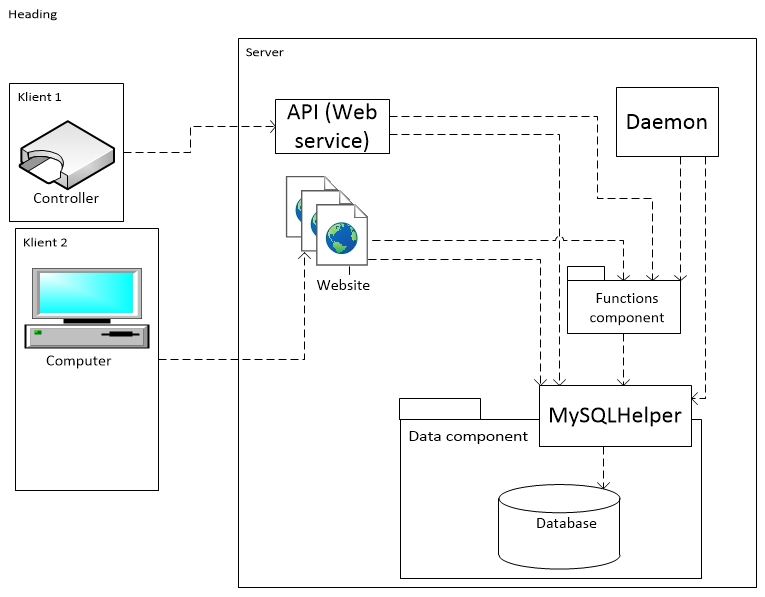
\includegraphics[width=1.25\textwidth,  angle=90]{images/serveroverview.jpg}
	\caption{system architecture}
	\label{fig:serveroverview}
\end{figure}

In the following chapters design and implementation of the web site, web service, deamon and database will be presented.

 



	\chapter{The Database}
\label{chap:database} 
In this chapter the database design and implementation hereof are explained. We will presents the ER-schema with our design and explain some of the design decision. Then we will shown the database scheme created from the implementation and explain some of the implementation decisions there have been made. Code samples will be shown from the function that update the simpler objects and finally there will be code from updating a rule.  
  
\section{Design}
\label{sec:DBdesign}
In the parent control system there are seven essential objects; control system, profile, tag, controller, chore, rule and permission. 

\begin{description}
	\item[Control system] is identifying the individual system and all of the other objects are connected to a control system.
	\item[Profile] is a representation of a specific person in the control system. The person can either be a child or the parent, but this should be distinguishable.
	\item[Tag] identifies the physical tag that a profile uses to activate the controllers. A tag is identified by the serial number of the physical tag.
	\item[Controller]	is an object representation of the physical controller and like the tag it is identified by the serial number of the physical controller.
	\item[Chore] is a representation of a house chore which can be carried out by a child (profile) which then gets points as a reward.
	\item[Permission] is representing restrictions on a controller which some of the profiles need to abide by. 
	\item[Rule] is representing other restrictions or rules that cannot be expressed by the permission. A rule consist of some conditions that need to be meet before some actions should be taken as explained previously in section \vref{sec:rule}. 
\end{description}

From the former description the database design is made. It is represented in an ER-diagram in figure \ref{fig:ERdiagram} where the cardinality ratio is expressed in Chen notation\citep{DatabaseKilde}. It should be mentioned that the design of a rule in the database is based on the first design of the rules, which can be found in appendix \vref{appendixFirstRuleDesign}. The reason for not using the final design is that it was changed fare into the implementation phase and the first database design does still support the final design of rule. 

\begin{figure}
	\centering
		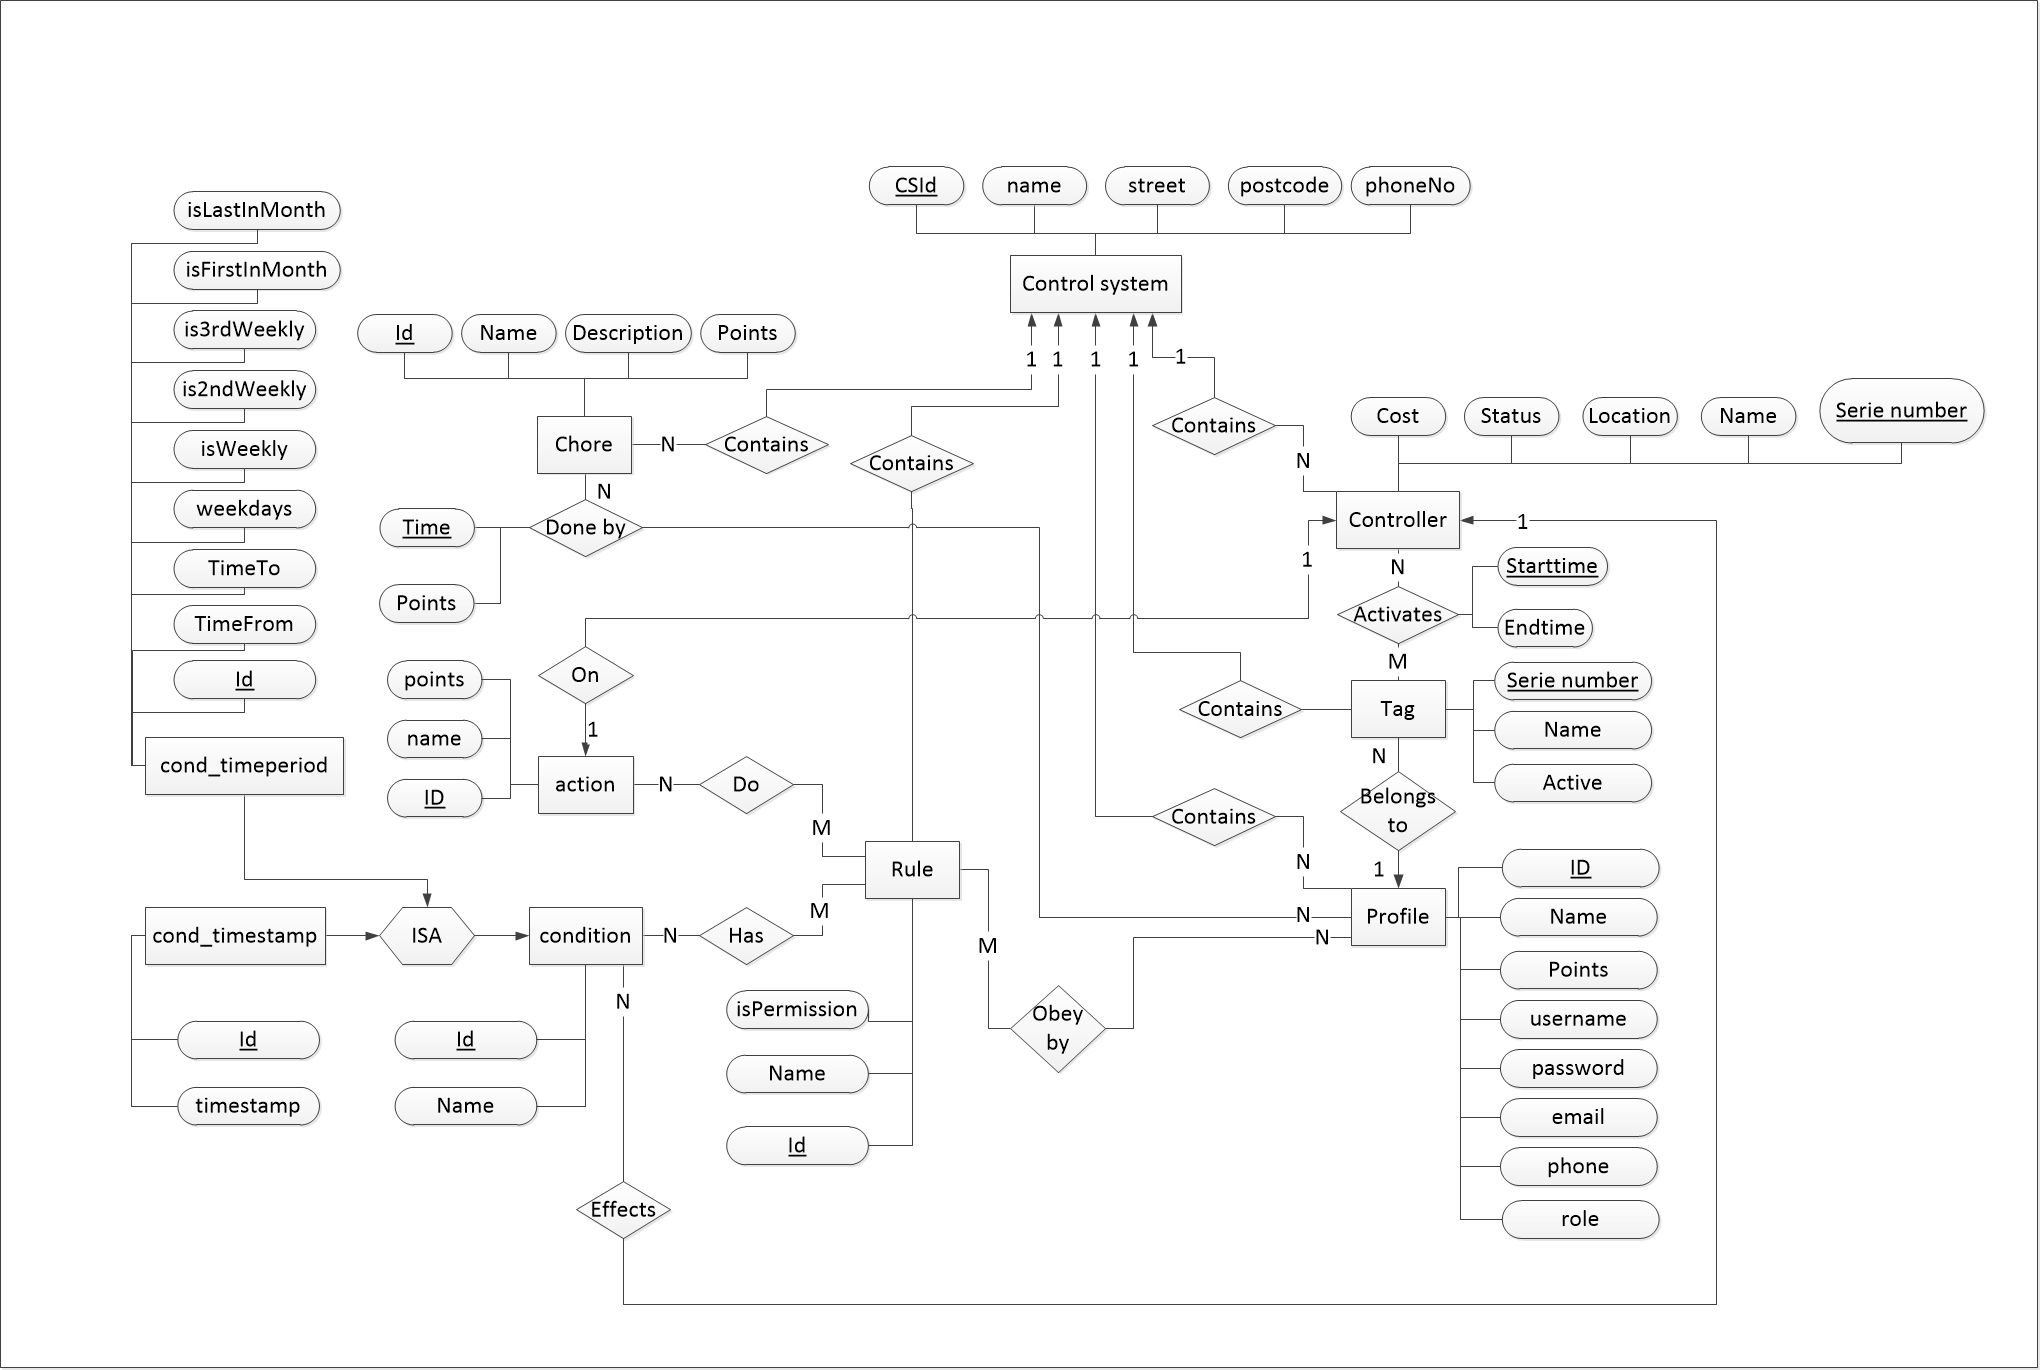
\includegraphics[width=1.50\textwidth,  angle=90]{images/ERdiagram.jpg}
	\caption{ER schema of the database design}
	\label{fig:ERdiagram}
\end{figure}

In the ER-diagram it should be noticed that Permission is absent. The reason is for every permission that could be made then there is an equivalent rule. Therefore the data representation of Permission is the same as Rule. However, on the website the two should be represented differently and so the attribute \texttt{isPermission} have been added to Rule which will differentiate the two.

Another observation from the diagram is the condition of a rule. The condition can be one of three representations. The first is the simplest because it is just the Condition. The second is Condition and a timestamp which is the \texttt{cond\_timestamp} in the design in figure \ref{fig:ERdiagram}. The last representation is Condition, a time period, and a representation of when it is valid, which in the ER-diagram is \texttt{cond\_timeperiod}. The type of condition that should be used, can be distinguished by the condition name. If the name is \texttt{Timestamp} it should be cond\_timestamp, if it is \texttt{Timeperiode} then it is cond\_timeperiod and any other name it is only the Condition. 

Notice if the database design had been designed from the final design then the table \texttt{cond\_timestamp} would not have been in the design.
After the database design had been completed it was implemented into a MySQL database.  

\section{Implementation}

The database design has been implemented in a MySQL database and the result can be found in figure \ref{fig:databaseDiagram}. In the implementation of the database redundancy and anomalies is to be avoided and null values reduced. 
The mapping from the ER-diagram to the relation representation in the database is a basic mapping according to the relations $1:1$, $n:1$, $n:m$ except for Condition which is clarified in the following section. \citep{DatabaseKilde}

\begin{figure}
	\centering
		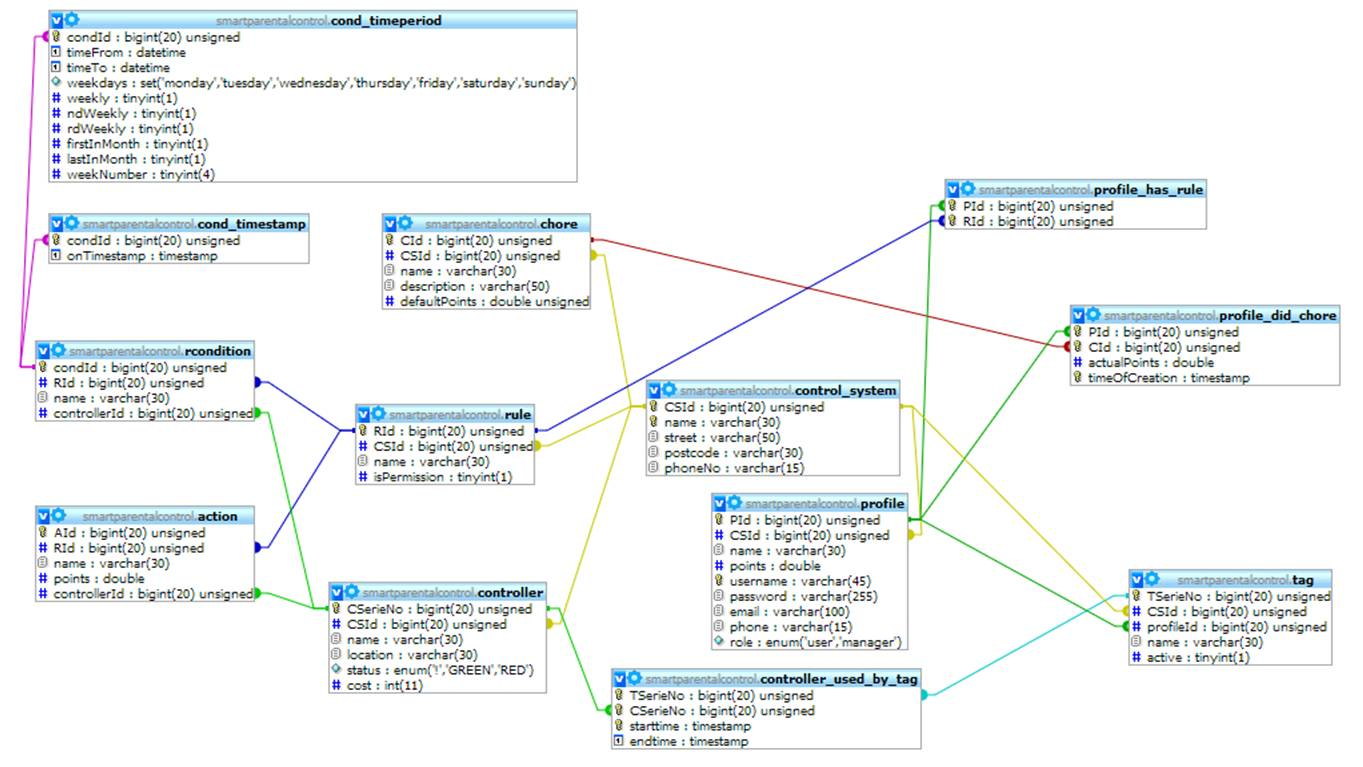
\includegraphics[width=1.50\textwidth,  angle=90]{images/databaseDiagram.jpg}
	\caption{The Database implementation}
	\label{fig:databaseDiagram}
\end{figure}

\subsection{Mapping of Condition}
\label{subsec:mappRule}
%sql or diagram
The relational modeling of Condition is more advanced because it uses generalization and as such there is a implementation choice to be made. There are four typical methods of how to deal with generalization and a solution of using each method is described below.\citep{DatabaseKilde}

\begin{description}
	\item[Using main classes,] then Condition is split up into three tables rcondition, cond\_timestamp and cond\_timeperiod where all attributes in Condition are repeated in each table. An disadvantage of using this method is in querying because it is possible to go though all three before finding the wanted data.
	\item[Using partitioning,] there are three tables rcondition, cond\_timestamp and cond\_timeperiod. The common attributes are in Condition and via an id the possible additional data can be found in either cond\_timestamp or cond\_timeperiod.
	\item[Using full redundancy,] it is much like the first, but all conditions from cond\_timestamp and cond\_timeperiod are also represented in Condition, without the additional data. As the name suggest this causes redundancy which is best to be avoided.
	\item[Using a single relation,] such that there will be a single table with all attributes from Condition, cond\_timestamp and cond\_timeperiod in the ER-diagram. It is easy to use but it will increase the number of null values. 
\end{description}

As can be see in the figure \ref{fig:databaseDiagram} the partitioning option is used in our implementation since it does not causes any redundancy or null values and it is easier to search for conditions compared to using the main classes. However, using partitioning there will be some challenges in making the functions to insert, update and get data about the rules, as will be explained in section \vref{subsec:dbRule}.\\\\

There have also been made an important decision about how to deal with deletion of data from the essential tables and this is explained in the following section.
 
\subsection{Deleting in the database}
%delete cascade
When a tuple in one of the tables control\_system, profile, tag, controller, chore, and rule should be deleted it will likely affect data from another table because of the foreign keys. We have made an intentionally decision to use \texttt{ON DELETE CASCASED} with all foreign keys, because in any case when deleting a tuple from the essential tables its history is irrelevant and should be deleted.\\
\\
As a consequence of this decision if a control system is deleted then every profile, tag, controller, chore, and rule that is connected to control system will be deleted. If a profile is deleted then this profile's tags will be deleted including all of its history, such as when the tag have been used to activate the controllers, or when the user have done a chore.
 So it is very important that when data is to be deleted then it should not be regretted later.  \\\\

However, for anything to be added, updated or deleted by the user the website need a connection to the database which is done through the class MySQLHelper. 

%sql Helper class
\subsection{MySQLHelper class}
The website and API for the controllers connect to the database by using a PHP class MySQLHelper, which establish a connection and send queries to it. The class have a construct and destruct that respectively establish the connection and close the connection to the database. The queries also go through this class in at least one of these methods:

\begin{description}
	\item[insertInto] this makes a SQL string to insert into the database.
	\item[update] this make a SQL string to update data in the database.	
	\item[delete] this make a SQL string to delete data in the database.
	\item[query] this make a SQL query string.
	\item[executeSQL] this sends the query to the database and returns the result. All of the above uses this method.
\end{description}
  
It is also possible to control the transactions through this class by disabling the auto-commit of transactions and then manually commit when it is necessary. \\\\

This class is used by several functions that are connected to the website, API and Daemon. In the following section we present the more interesting of them, how to update rules. 

\subsection{EditRule from the Function Library}
\label{subsec:dbRule}
%if someday our repport gets to long this can be cut out or reduced
This system also have a function library which can get, insert, update or delete data from the database. Among these functions are e.g. \texttt{simpleInsertIntoDB} and \texttt{simpleUpdateDB} that is used to insert and update the essential tables with the exception of Rule. Insert and updating a rule is similar but the latter is the more interesting so it will be this sections focus. 

As stated previously in mapping of a rule in subsection \vref{subsec:mappRule}, there would be some challenges to make the insert and update functions. This is partly due to the fact that the data of a condition  is one of two alternative: condition, condition plus timestamp  or condition plus timeperiod as was explained in section \vref{sec:DBdesign}. However, in the newer design of a rule the condition plus timestamp is removed which makes it easier, but the problem still exists. In update it is also a challenge that each condition and action can be removed, add or updated which all should be handled together and this will be explained further in this section. 

The function to update a rule is called editRule and it also uses some other function as described below:

\begin{description}
	\item[addAction] from a rule id and an object of type Action it adds an action to the rule.
	\item[editAction] from an object of type Action it updates the attributes in the database.   
	\item[addCondition] from a rule id and an object of type Condition adds a condition to the rule.
	\item[editcondition] from an object of type Condition it updates the attributes in the database.   
\end{description}

The editRule has three inputs a Rule object, an array with Condition objects, and an array with Action objects. First the rule data will be update and then each condition and action must also be updated. 

However, when updating an action and especially a condition the changes can have different characteristics as listed below. This is also in the decision diagram in figure \ref{fig:updateRule}.

\begin{itemize}
	\item a new condition or action is added.
	\item a condition or action need to be deleted.
	\item an existing condition or action is to be updated with no structural change in the database.
	\item an existing condition or action is to be updated but with a structural change in the database.
\end{itemize}

With a structural change it is meant that the name of the condition or action has been changes and this change can influence e.g. whether cond\_timeperiod or cond\_timestamp should be used. As a result it have been decided that in this case the old condition should be deleted and the new be added anew. A structural change should not happen for an action, but the functions are still able to handle it in the same way as a condition.

\begin{figure}
	\centering
		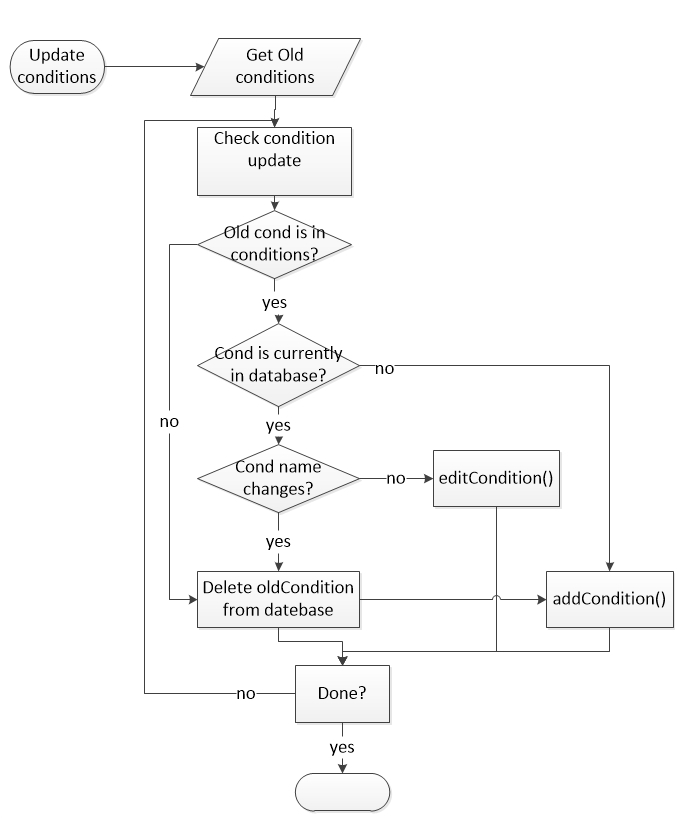
\includegraphics[width=0.75\textwidth]{images/updateRule.jpg}
	\caption{updateRule}
	\label{fig:updateRule}
\end{figure}



%
%The code sample in \ref{code:UpdateRules} is from the update handling of condition and the it is similar to handle the actions. First the old conditions id are need such that they can be compared to the ids of the Condition objects from the array \$arrayOfCondition, see line $2$. 
%Then foreach old condition id we will look thourgh the new id and if it found and the name are not to be changed then we call editcondition with the updated condition object and remove this object from the array of condition, see line $4-20$. 
%From line $22-26$ it is shown that the tuple with the old id is removed if no match was found among conditions in the array or if a match was found but the name are to changed. Now all the condition that was intended to be deleted is gone and finally the remain objects is then add or re-add from the array with addCondition, see line $28-40$.
%
%
%\begin{lstlisting}[language=PHP, label=code:UpdateRules, caption=editRule code sample]
%//SELECT condId AS id FROM rcondition WHERE RId = ($ruleData->RId)
%$CondIdResult = $db->query($theColumns['Rcondition'][0].' AS id', $theTables['Rcondition'], $theColumns['Rcondition'][1] . " = " . $ruleData->RId );
				%
	%while($row = mysqli_fetch_assoc($CondIdResult))
	%{
		%$StillExists = false;
		%foreach($arrayOfCondition as $key => $cond)
		%{
			%if($row['id'] == $cond->condId && $cond->name == null)				//edit the condition in db
			%{
				%$StillExists = true;
				%$tempresults = editCondition($cond);
				%unset($arrayOfCondition[$key]);
				%if(is_string($tempresults))
				%{
				%//if not bool then it is an error message
					%return $tempresults;
				%}
			%}	
		%}
		%//row id is not among the updated condition or cond_name not null so delete 
		%if(!$StillExists)
		%{
			%$db->delete($theTables['Rcondition'], $theColumns['Rcondition'][0] . " = " .$row['id']);
		%}
	%}
	%//add the remaining condition to db
	%if($arrayOfCondition != null )
	%{
		%foreach($arrayOfCondition as $cond)
		%{
			%//if a new condition should be added then make condition here
			%$tempresults = addCondition($ruleData->RId, $cond);
			%if(is_string($tempresults))
			%{
			%//if not bool then it is an error message
				%return $tempresults;
			%}
		%}
	%}
%\end{lstlisting}

\subsubsection{Status on Database and Function Library}

The database and the functions mentioned have all been made prior to when the decision of the rule's design changed. The functions which uses condition can now be further improved but this will not be done because it is not a priority since these functions still meet the requirements of the system.

Up till now the rules could have several conditions and actions but late in the implementation of the Website we have decided to only allow one action and condition per rule to get a more user-friendly website, more about this decision can be found in section \vref{subsec:rulesWEB}. Most functions are still implemented on the first design so they can handle several conditions and actions. 

However, a few functions can only work with one condition and action per rule. An example is the function that checks whether a user can use a media, called $db\_rules\_user\_can\_turn\_device\_on$. If the implementation of rules on the website is changed a new version of these functions need to be made.

	\chapter{The API}
This chapter will explain the design and implementation of the API for this project.
\section{Design}
The API started with one clear goal, to be the middleman between the controllers and our database. The API's main purpose is to abstract away the need for the controllers to work directly with the database, along with it meaning more security for the database. With this in mind the API should also be as simple as possible, which lead to the API having only three actions. The three actions are \texttt{status}, \texttt{turn on} and \texttt{turn off}. \\
\texttt{Status}' job is a way for the controller to check up on if there have been any changes in time remaining for the user. This means that \texttt{status} has to check if there are any rules that will cut the user off before they run out of points. If there are no rules that interferes then it should calculate the time remaining again for the user and return that. \\
\texttt{Turn on}'s main function is for the controller to request for it to turn on. This means that \texttt{turn on} should check to see if the controller can be turned on, calculate the time remaining, turn on the controller inside the database and finally return that. When checking to see if the controller can be turned on, \texttt{turn on} should check both that the user has enough points for at least a minute of on time and that there are no rules that are preventing the controller from turning on.\\
\texttt{Turn off}'s main function is for the controller to tell the API that it wants to turn off. This means that \texttt{turn off} should check if it is the same user who is turning the controller off and if it is not the same user report an error. \texttt{turn off} should then calculate the time spent on the media and calculate how many points to remove from the user and then remove it. Finally it should return the time spent and the points removed. \\
\autoref{fig:turnOnAPI1} shows the flow of how the API checks if a controller can turn on. First it checks if the controller id and tag id is valid. It then checks if any rules or permissions prevent the controller from turning on or user from turning on the controller. Then it checks if the device is already off and if the user has enough points to turn the controller on. If any of the checks are false an error is returned, otherwise it turns on the controller in the database and returns the result to the controller.

\fixme{use figures for at least one: you can use the ones below:}

\begin{figure}[!h]
	\centering
		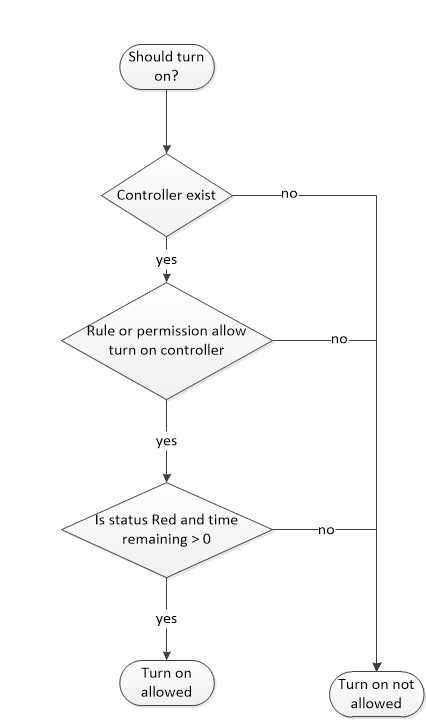
\includegraphics{images/turnOnAPI1.jpg}
	\caption{Flowchart showing how turn on works}
	\label{fig:turnOnAPI1}
\end{figure}
 
\section{Implementation}
The API has been implemented on top of the Slim routing framework and PHP. The reason for this framework is that it makes it quicker and easier to make an API, while also making it easy to add additional endpoints. The communication between controllers and the API are done using HTTP and JSON. JSON has been chosen because of its almost universally support and its small overhead. This means that the communication is easy to implement, and easy to port to additional platforms if necessary. Calling the API is as simple as navigating to a website. Parameters to the API is done using custom GET messages. An example of a call to get status could be \texttt{http://example.com/api/api.php/turnOn/123/234} where \texttt{example.com} is the domain where the API is hosted, \texttt{123} is the controller id and \texttt{234} is the users tag id. An overview of the available calls and their parameters can be seen in \autoref{tbl:apicalls}.

\begin{table}[!h]
\begin{tabular}{| l | l | l |}
\hline
Call & Parameters & Return values \\
\hline
/status/ & cId & status, action, timeRemaining \\
\hline
/turnOn/ & cId, tId & status, timeRemaining, error \\
\hline
/turnOff/ & cId, tId & status, timeSpent, pointsRemoved, error \\
\hline
\end{tabular}
\caption{A table containing the available calls of the API. A legend of the keywords can be found in \autoref{tbl:apilegend}}
\label{tbl:apicalls}
\end{table}

\begin{table}[!h]
\begin{tabular}{| l | p{9cm} |}
\hline
Keyword & Description \\
\hline
cId & The id of a controller \\
\hline
tId & The id of a users tag \\
\hline
status & Status of the API call, \texttt{OK} if successful, \texttt{ERROR} if failure \\
\hline
action & The action the controller should take, \texttt{none} if no action should be taken \\
\hline
error & A description of the error that has occurred if any has, error is omitted from the JSON if there was no errors \\
\hline
timeRemaining & The amount of time before the controller should turn itself off in minutes \\
\hline
timeSpent & The amount of time the controller was one in minutes \\
\hline
pointsRemoved & The amount of points removed from the user \\
\hline
\end{tabular}
\caption{A table containing a legend of the keywords used in \autoref{tbl:apicalls}}
\label{tbl:apilegend}
\end{table}

	\chapter{The Daemon}
\label{chap:daemon}
This chapter will explain the design and implementation of the daemon of this project. A daemon is a computer program that runs in the background continuously without any input from a user.
\section{Design}
The daemon has one main job, to activate rules that require action at a specific or recurring time. Right now there is only one such action, \texttt{Add points}, which when activated has to add points to a given users profile. This cannot be done using a normal website because of the time requirement that the points have to be added at the right time. Further things that the daemon should handle could be such things as \texttt{Activate tag} and \texttt{Block tag} if these were added as actions to the rule system. \autoref{fig:daemonflowchart} shows how the flow of the daemon should work. It should check rules every minute if they should activate, and activate those who should, doing the action specified.

\begin{figure}[!h]
	\centering
		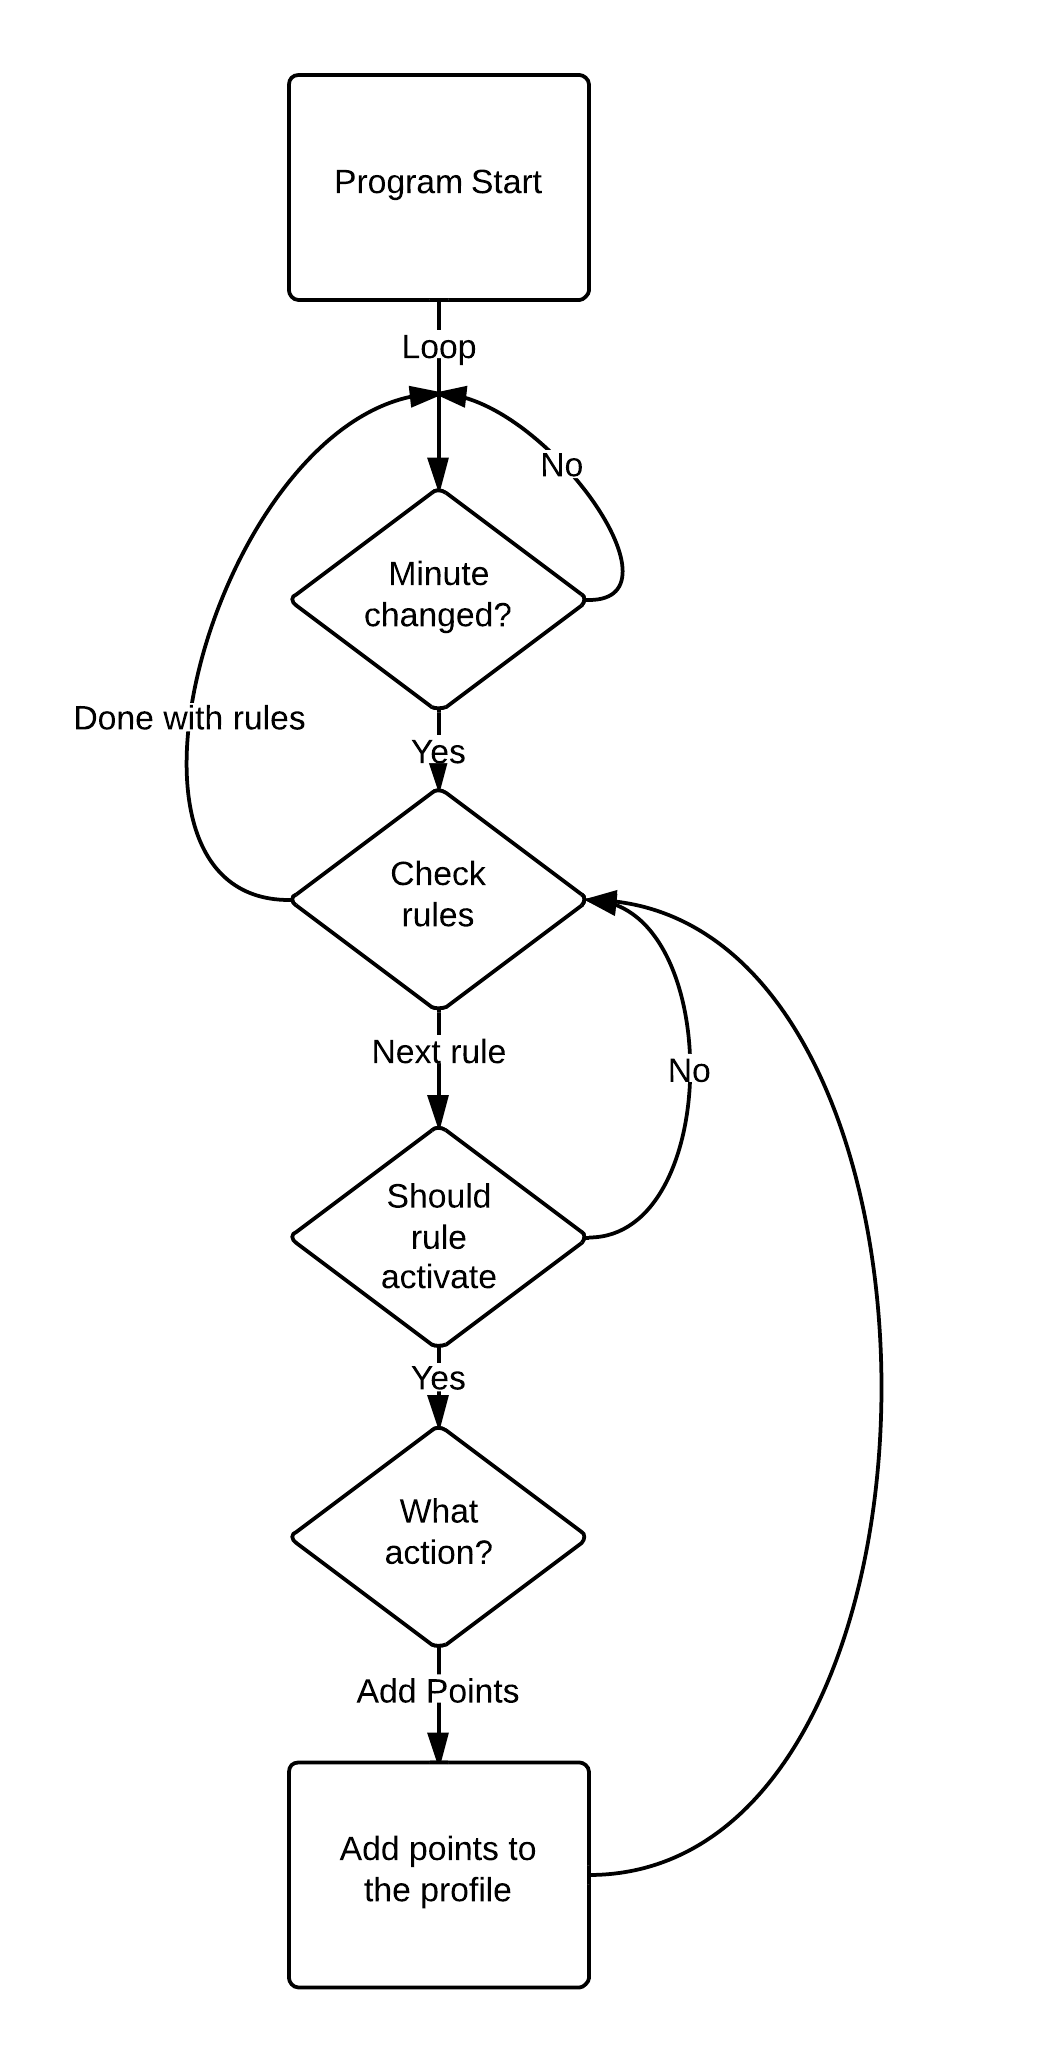
\includegraphics[width=0.65\textwidth]{images/daemonflowchart.png}
	\caption{Flowchart showing how the daemon should work}
	\label{fig:daemonflowchart}
\end{figure}

\section{Implementation}
Because daemons usually run all of the time, it is not appropriate to be implemented in PHP, as PHP is not meant to run continuously. The choice has then fallen on Python as the programming language. The reason for this choice is that Python is a dynamic language like PHP that is quick to build prototypes in. Unlike PHP, Python is meant to run continuously while PHP is meant to run and exit. \\
The daemon like the website communicates with the database directly. The daemon is set up to check rules that have actions, conditions and profiles attached. It checks if these rules should activate based on their \texttt{time from} and \texttt{time to} timestamps as well as their repeatability options. There are four ways a time period condition attached to a rule can activate based on weekday, week, last/first in month and time stamp. Weekday is activated when the time period has weekdays selected but not any repeatability options enabled, i.e. the current weekday should match one of the selected ones and the current date and time should fall between \texttt{time from} and \texttt{time to}. Week activates based on the difference between the \texttt{time from} date and time, and the current date and time. This means that the absolute week is the one used to calculate weekly, biweekly and triweekly. Last/first in month is based on weekday, if the weekday selected is the current day then the condition activates if the current day is the first/last monday/tuesday/.. of the month. Lastly the condition activates if the current time and date is between \texttt{time from} and \texttt{time to} and the condition has no repeatability enabled. \\
The daemon checks rules every minute, by keeping check on the last minute the rules was checked at, and if it has changed, then it checks the rules. This method was favored instead of a simple sleep for 60 seconds as there were possibilities where the daemon would not check a minute, e.g. if the daemon started checking rules 40 milliseconds before a new minute, the daemon would take 50 milliseconds to check rules, then sleep for 60 seconds, this would make the daemon skip a check on a minute which could make conditions not activate when they should.
	\chapter{Design of the Controller}
This chapter is focused on the controller system of the Media-Online Management system. The controller system is the hand and mouth of the MOM system. Handling the every day use of MOM system as activating and restricting users from media devices.\newline
This chapter is focused on the controller of the Media-Online Management system. The controller consist of a tag reader and power control device which is disgusted in this chapter but when mentioning controller both is implied. \newline
The design and functionality of the prototype controller will be presented in parallel to the designed end product. \newline

\section{Product Design}

The product design section is the vision of the system as a finised product. Figure \ref{fig:Power&Tagdevice} is the illustation of the embedded system called the controller system. The controller system is connected to the server though a wifi connection to insure that a ethernet outlet don't need to be a every media devise.  
The controller is two devices, detection device and power control device.

\begin{figure}[h]
	\centering
		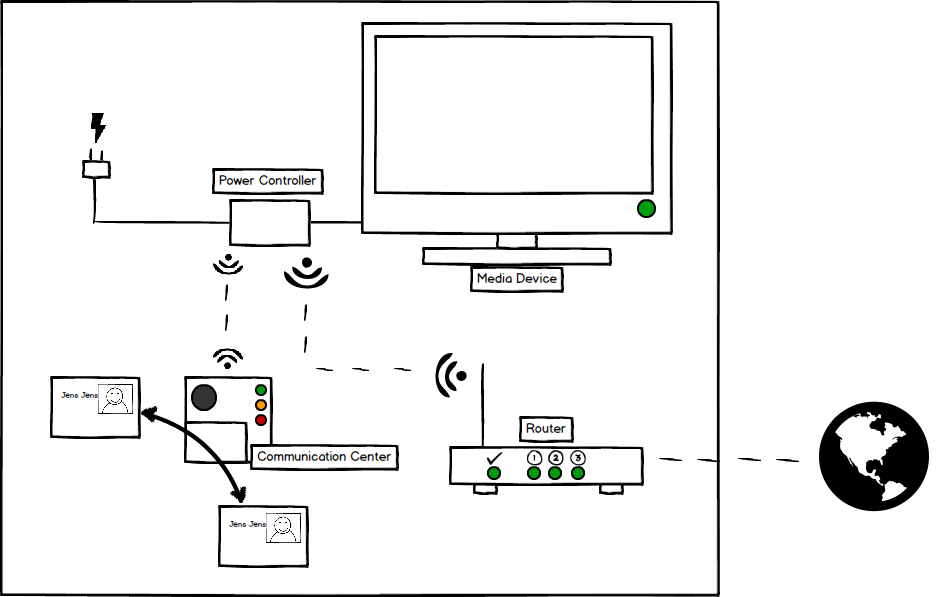
\includegraphics[width=1.00\textwidth]{images/Power&Tagdevice.png}
	\caption{Rich picture for Powercontrol and Tag reader}
	\label{fig:Power&Tagdevice}
\end{figure}

Detection device reads user tags when swiped over the detector device. This device is separated from the power control device to increase user friendliness. The power control device will be placed on the power cable to the media device will that not always be as accessible for the use if one want to scan a tag. Therefor shall the detection device often be placed infront of the media device to give the user friendliness.\newline
The other device is a powercontrol device which is located on the powerline to the media device and turns on and off the electricity when needed.\newline
The powercontrol device(PCD) is the brain of the two devices and is therefore to monitor the time usage of the media. It should also communicate with the server and detection device. \newline
The detection device(DD) should also inform the user who is trying to activate a media of whether the activation has been approved or declined by the server.
%The detection device(DD) also works as an information communicator to the user, on the state of the connection to the server about acceptance/decline of log-in. \newline    

\subsection{Senario Design}
\label{subsec:senarioD}

The system has been designed on multiple scenarios and the criteria of communication to the server and user. The flow chart \ref{} is an overview of the action and communication between server, the controller system and user. The flow chart illustrat the controller system:

\begin{itemize}	
	\item Register user tags and get user rights from server. 
	\item Adminstrat user rigths according to server information.
	\item Moniter the connection wifi to server and handele the exseption op disconnected. 
	\item Regulate the power to a device recording to senario.
	\item Manage the time usaged and user restigtions.
	\item Communicat system status to user.
\end{itemize}

\fixme{indsæt Flowcart af systemet}

The development was done by asking and answer questions to the system in different senarios.\newline
The flow chart is a combined answer here of. \newline

\textbf{Setting up and turning on the system.} \newline
In the final design the PCD will receive the information about the WiFi connection from USB drive.
If the information on the USB is wrong or not received then a restart button is included to redo the procedure.  \newline
The PCD will then connect to the WiFi network and add the controller to the database in his MOM system. If the connection is not found a message is send to the DD. \newline 
DD indicates that there is no connection by showing a constant red light. The communication protocol can be found in the appendix \vref{appen:lights}.\newline When the connection is established then the DD is ready to read user tags.\newline

However, this design will not be implemented in this project. Instead there is a wired connection to the internet and the controller need to be manually added into the database.

\textbf{Detection of connection issues and status changes.} \newline
The connection to the sever is tested by a routine call every five minutes from the PCD to the server. In this call the PCD will receive information on when the media should shutdown based on a rule or the user's remaining time. This insures that if any changes in the remaining time or the rules which will influences when the media should shut down then it will still be handled.
%This insure that there is a connection each five minutes and if any changes in rules or in the time the user may spend on the media. 
In between those calls the PCD will check for a tag from the DD. If the PCD is disconnected from the server that is informed to the DD and to the user.  \newline
	
\textbf{Logon/logoff media divice.} \newline
When a tag is read by the DD the PCD will receive the tag id which is then formed into a log-in message and send to the web servers API. however this is only if no one ready is logged on the media device in the MOM system. The PCD will then get a message about whether the user has permission to use the media from the API. If the user has permission then the PCD should direct power to the media, then save the tag id in local memory and receive the remaining time from the API. The DD should indicate whether the user is approved to use the media.\newline 
To log-off the user will swipe ones user tag again and the PCD receive the same tag id that is stored in the local memory. The PCD will then switch off the power to the media and send a log-off message to the API. \newline
If another user wants to take over the usage of the media then the PCD should try to log-in with the new tag. If this is declined then the DD should then signal this and keep the old user logged on. If it is accepted then the server should overwrite the previous user and PCD will receive the information for the new user with out turning the power off and then on again.\newline 
The functionality of switch users is not implementet in the current prototype.\newline

\textbf{Server disconnection under use.} \newline
A disconnection from the server is either found under the regular status call after each five minutes or at a log-on/log-off call. A disconnection will lock the device so only the current user can use the media until the PCD is reconnected with the server. The server discovers the lack of connection when there have not been a status call from the device in five minutes. The disconnection is translated to a log-off the media at the server side. 
The user will not be logged off by the controller but will be able to use his time according to the last status. If the user want to log-off in a period where there is a disconnection a time stamp is saved and will be sent to the server when the connection is reestablished. The media can also first be used again when the connection is reestablished. 
This procedure have the advantage that the user will not have to cut off the media in use if the connection is unstable. The user will also be able to use a another media with connection to the server.
The disadvantage is that the user has the possible to exceed the time restriction if there has been a change in the rules or the user's remaining time. \newline
The implemtation of exseption of disconnection in prototype is not as the descriped above. \newline 
	
	\subsection{Using the Ethernet Shield.}
\label{sec:ethernetshield}
\fixme{Mangler kort kommentar om hvorfor Ethernat er brugt istedet for en Wifi connection}
The Ethernet shield is the primary component in accessing the API as it allows for the Arduino to access the web as a client.
We use the Ethernet shield along with a JSON parser in order to make HTML requests on the web site that contains the system API and decode its responce.

The Ethernet Shield comes with an MAC address printed on the side which is used to automatically obtain an IP Address.
This along with the target server is established as global variables as seen in \autoref{EthStart} along with the Method call in \verb|Setup()| that establishes a connection with the LAN. All supplied from the Arduino Library \verb|Ethernet.h|.
\fixme{kunne være korte statement på sær funktioner for eksemple F står for når du printer} 
\fixme{linje 22, Hvad sker der så, er det bare en død Audrino?}

\begin{lstlisting}[frame=single, label=EthStart, caption=The Method Calls used to establish and maintain a connection.]
//The Mac Address declared.
byte mac[] = { 0x90, 0xA2, 0xDA, 0x0E, 0xC5, 0x94 };

//Our target Server that the API is called on
char server[] = "spcadmin.tk";

//When this statement is evaluated the Arduino connects to the LAN.
//This happens during Setup();
if (Ethernet.begin(mac) == 0) 
{
  //If the Evaluation returns 0 it fails and stops doing anything.
	Serial.println(F("Failed to configure Ethernet using DHCP"));
	while(true); 
}

//The following code us run in every loop through checkConnection() call to assure
//that the DHCP lease is renewed when needed.
Ethernet.maintain();
\end{lstlisting}

Whether the user tries to log in or out from the device, the Arduino will have to access the web server via the API.
The process is almost identical in either case and can be divided into two parts:
\begin{itemize}
	\item Connecting to the API.
	\item Parsing the servers Reply.
\end{itemize}

As seen in \autoref{pageConnect} the Device ID and the Tag ID is connected in a char array to form the url which complies with the action that is being performed. \fixme{connect this to the API implmentation}
Then in return the Ethernet Shield receives the HTML Page, and in \autoref{pageDecipher} the Arduino reads this information one byte at the time where all but the JSON string is stripped and stored in a char pointer.
When all the bytes have been through this progress the connection is closed and the JSON string is parsed the result of the action. This can be seen in \autoref{pageJSON}.
\begin{lstlisting}[frame=single, label=pageConnect, caption=Connecting to the Server and creating an HTML request.]
void turnOn(void)
{
  if(client.connect(server, 80))
  {
    Serial.println(F("Connected")); 

    client.print(F("GET /api/api.php/turnOn/"));
    client.print(devID);
    client.print(F("/"));
    client.print(useID);
    client.println(F(" HTTP/1.1"));
    client.println(F("Host: spcadmin.tk"));
    client.println(F("Connection: close"));
    client.println();
    
    Serial.println(F("Message Sent"));
\end{lstlisting}

\begin{lstlisting}[frame=single, label=pageDecipher, caption=Removing all but the important information from the website.]
while (client.connected())
{
  //Builds the JSON string from the data passed by the website.
  while(client.available()) 
  { 
    buff = client.read();   //Bytes are passed through the Ethernet Shield with client.Read();
    if(buff == '{')        //The JSON string starts with '{' and stops with '}'.
    {
      toggle = !toggle;
      *(on+i) = buff;
      i++;
    }
    else if(buff == '}')
    {
      toggle = !toggle;
      *(on+i) = buff;
      i++;
    }
    else if(toggle)
    {
      *(on+i) = buff;
      i++;
    }
  }
}
client.stop();
\end{lstlisting}

\begin{lstlisting}[frame=single, label=pageJSON, caption=The JSON Code Getting a value with a Token.]
aJsonObject* json = aJson.parse(on);
aJsonObject* statJson = aJson.getObjectItem(json,"status");
char * stat = statJson->valuestring;
\end{lstlisting}
	\subsection{Using RFID With The Arduino}
\label{sec:rfidsect}
\fixme{Mangler lidt mere start som der var i Using the ethernet shield.}
The Arduino board utilizes the SM130 by sending it commands and receiving replies through Digital Pins 7 and 8.
These pins are initialized using the library \verb|SoftwareSerial.h|.\\
\begin{lstlisting}
SoftwareSerial rfid(7, 8); //Sets up the Digital Pins 7 and 8 '
                           //Which the RFID reader Communicates through.
													
rfid.begin(19200); //This Method is called in the Setup() phase 
                   //of the Arduino Startup.
									 //It starts the Communication on the standard baud
									 //rate of 19200 bps, N, 8, 1.
											
\end{lstlisting}
\fixme{enten skal vi forklare hvad "`baud"' og hvad 19200 bps, N, 8, 1 står for.}		

These messages are a series of bytes sent one at the time in the form of Hexadecimals and in the context of an UART framed message. \newline
\begin{tabular}{|l|l|l|}
\hline \hline
Header: & 1 Byte & Must always be 0xFF.\\ \hline
Reserved: & 1 Byte & Must always be 0x00.\\ \hline
Message Length: & 1 Byte & The amount of bytes used on Command and Data.\\ \hline
Command: & 1 Byte & The Hexadecimal value of the command in question.\\ \hline
Data: & n Bytes & The bytes containing the data needed for the command.\\ \hline
Checksum: & 1 Byte & The combined value of all above hexadecimals.\\ \hline
\end{tabular}
The command messages needed we need to allow logging in with a tag are: 
\begin{itemize}
	\item Seek: The Module activates `anti-collision' and `Select Tag' so that it can catch a tag when it comes in range.
	\begin{itemize}
		\item Message Length:Seek has a message length of 1 byte as there is no accompanying data.
		\item Command: 0x82 is the Seek Command.
	\end{itemize}
	\item Authenticate: When a tag has been found this command authenticates a single block of data on the RFID Tag, which must be done before it is read.
	\begin{itemize}
		\item Message Length: The authenticate command message is 3 bytes long as it needs 2 databytes.
		\item Command: 0x85 is the Authenticate Command.
		\item Data Byte 1 (Block Number): Tells the SM130 which data block on the tag is to be authenticated.
		\item Data Byte 2 (Key Type): Informs which type of key should be used to authenticate with. The SM130 has 2 Key types to authenticate with (A and B), and 15 slots for each to store individual keys. We use the build in 0xFF which authenticates with Type A and the transport key ``FF FF FF FF FF FF''.
	\end{itemize}
	\item Read Block: Reads a previously Authenticated block of data on the RFID Tag, The data contains the Tag ID.
	\begin{itemize}
		\item Message Length: The Read Block Command message is 2 bytes long as it needs information on what block is to be read.
		\item Command: 0x86 is the Read Block Command.
		\item Data Byte (Block Number): Tells the SM130 which data block on the tag is to be read.
	\end{itemize}
\end{itemize}

As an example \autoref{RBCE} is the code run when sending the Read Block Command to the SM130.
\begin{lstlisting} [label=RBCE, caption=Example of the Read Block Command from the code point of view.]
void read_block_RFID(void)
{
  //Read Block Command in UART, sent to the SM130. The Block needs to be Authenticated beforehand.
  rfid.write((uint8_t)0xFF); //Header: 1 byte, must always be 0xFF.
  rfid.write((uint8_t)0x00); //Reserved: 1 byte, must always be 0x00.  
  rfid.write((uint8_t)0x02); //Message Length: 1 byte, both for Command and Data (Here: 2 bytes).
  rfid.write((uint8_t)0x86); //Command: 1 byte, 0x86 is the Read Block Command
  rfid.write((uint8_t)0x01); //Data(Block Number): 1 byte, read block nr 0x01. 
  rfid.write((uint8_t)0x89); //The Message Checksum.
  delay(10); 
}													
\end{lstlisting}


On being given a command the SM130 will send a response from which you can tell if the command has been successfully performed or not.
In the code this information is saved on a char array by the parse method seen in \autoref{arduinoparse}. 
On `Seek' and `Read Block' we determine the success by reading the slot containing the length of the Message, while on the Authenticate command the Data slot is read to determine success.

\begin{lstlisting} [label=arduinoparse, caption=The method used to read the SM130's response.]
void read_block_RFID(void)
{
void parse_response(char PH[], int length)
{
  for(int i=1;i<length;i++)
  {
    PH[i] = 0;
  }
  
  while(rfid.available()) //This whileloop runs so long as there is still bytes to be read. 
  {
    if(rfid.read() == 255) //Checks for the Message Header.
    {
      for(int i=1;i<length;i++)
      {
        PH[i]= rfid.read(); //For the Length of the expected UART message, Add bytes to the Array.
      }
    }
  }
}
}													
\end{lstlisting}


\fixme{Ryk tabelen længere op da det vil give mere mening til alle henvisninger til bytes.}
\begin{tabular}{|l|l|}
\hline
\hline
& The RFID output in UART for seeking for tag:\\
&  On 'Tag Found'. (The length would be 0x06.)\\
\hline
Slot 0-3 & Contains the message "Header", "Reserved", "Length" and\\
& "Command".\\
Slot 4 & Contains the tag type. \\
Slot 5-8 & Contains the data stored in the block.\\
Slot 9 & Contains the Checksum.\\
\hline
&On 'no tag found'. (The Length is 0x02.)\\
\hline
Slot 0-3 & Contains the message "Header", "Reserved", "Length" and\\
& "Command".\\
Slot 4 & Contains the Error Code.\\
& \indent - 0x4C: `L' Command in progress.\\
& \indent - 0x55: `U' Command in progress but RF field is off.\\
Slot 5 & Contains the Checksum.\\
\hline
\hline
&The RFID output in UART for Authenticating a Data block.\\
\hline
Slot 0-3 & Contains the message "Header", "Reserved", "Length" and\\
& "Command".\\
Slot 4 & Contains the Status/Error Code.\\
& \indent - 0x4C: `L' - Login Successfull.\\
& \indent - 0x4E: `N' - No Tag Present or Login Failed.\\
& \indent - 0x55: `U' - Login Failed.\\
& \indent - 0x45: `E' - Invalid Key format in E2PROM.\\
Slot 5 & Contains the Checksum.\\
\hline
\hline 
& The RFID output in UART for reading a block: On a success.\\
& (The length would be 0x12.) \\
\hline
Slot 0-3 & Contains the message "Header", "Reserved", "Length" and\\
& "Command".\\
Slot 4 & Contains the number of the block read. \\
Slot 5-20 & contains the data stored in the block.\\
Slot 21 & Contains the Checksum.\\
\hline
&On a Fail (The length is 0x02.)\\
\hline
Slot 0-3 & Contains the message "Header", "Reserved", "Length" and\\
& "Command".\\
Slot 4 & Contains the error code:\\
& \indent - 0x4E: `N' No tag present.\\
& \indent - 0x46: `F' Failed to read.\\
Slot 5 & Contains the Checksum.\\
\hline
\end{tabular}
	\subsection{ArduinoDesign.}    
\fixme{Indsæt flowchart}

Flowchart is the current level of the prototype as is very similar to figure \ref{fig:Power&Tagdevice}.

Therefore  the Ardurino hardware should be seen as replaceable by another controller device in this system. 
	\chapter{Admin Web Interface} %\fixme{mention somewhere that dashbaord, calendar and graf has static data}
\label{chap:website}
This chapter goes into details about the design and implementation of the website used to administrate Media-Online Management (MOM).

\section{Design}
%Interface Design
%What you can do from the website, and how
The requirements for the website is discussed in \autoref{section:momswebsite}.
These requirements made the basis for deciding what pages should be created and what each page's functionality should be. During the designing of the website it was aimed to fit all relevant information into each page.\\
All pages have been designed on the blackboards, where inconsistencies was discovered, new navigation paths and learn about how concepts such as rules should be implemented.\\
Next is a short overview of what pages were designed and their purposes.\\
\\
\textbf{Dashboard} is used to get a quick overview of relevant data. The overview is customizable so that each parent can decide what information is most relevant for them.\\
\\
\textbf{Devices} is used to get an overview of which controllers and tags is registered within their MOM system. It also is the only way to navigate to the Add Tag/Controller and Details Tag/Controller pages.\\
From this page it is also possible to deactivate a tag, meaning the owner of that tag, can no longer log in with it.\\
\\
\textbf{Devices - Details Controller} is used to display, delete and change information about a controller. A user can only access controllers that is registered to his system.\\
\\
\textbf{Devices - Details Tag} is used to display, delete and change information about a tag. A user can only access tags that is registered to his system.\\
\\
\textbf{Devices - Add Controller} is used to add controllers to the user's system. In order to add a controller the user must add a unique key found on the controller, this is then checked towards a database of available keys.\\
However it has not currently implemented this way of validation, but it would be the right way to go in order to commercialize the system and ensure security for our users.\\
\\
\textbf{Devices - Add Tag} is like Add Controller, except with tags. Also in order to register a tag, a user must be dedicated to this tag. The one registering a tag, will be meet by a list of current users in the system. This means that in order to apply a tag, one must first create a user, then register a tag.\\
\\
\textbf{Users} is used to get an overview of users in one's system. It is also used to navigate to Create User and User Details.\\
\\
\textbf{Users - User Details} is for viewing details about a user. It is also used to change information about a user, however it is only possible to change information, if your user is of a manager-role, or if you are the owner of that profile.\\
\\
\textbf{Users - Create User} is as the name suggests, used for creating a user. The system has been made ready for children to login to the system already now. There is not any feature that requires the children to log in to the system as of yet, but a feature might utilize this later on.\\
\\
\textbf{Users - Chores} is used to get an overview of available chores, and for easy rewarding of already created chores. When a chore is done, the parent should go to this site, and simply select a child and press a button to give them the assigned reward of the chore.\\
Chores will also have a subsite for creating chores.\\
\\
\textbf{Users - Rules} is where parents can get an overview of rules and create them for their system. Great care has been taken to help users in creating rules, by making a step by step procedure. Starting with making the user choose what sort of action they want to achieve and thereafter choose the sort of condition they want to set, since actions only match certain conditions. This should limit some of the confusion about the rules. For more information about rules, actions and conditions see subsection \vref{sec:rule}.\\
\\
\textbf{Users - Permissions} is designed for an easier way to think of rules, in relation to what devices which child is allowed to use.\\
It was decided to create this permissions page, because permissions is an essential part of even the smallest of systems, you can create a system without rules, but not without permissions.\\ %This tool gives the parents an easy way to limit their child’s usage, by deciding devices can not be turned on after a certain time.\\
\\
\textbf{Graf} page is intended for viewing statistics, such as how much have a controller been active, how is a users usage of media divided and so forth.\\
\\
\textbf{Calendar} has two purposes. It serves as a graphical presentation of rules, in the sense that it shows when a rule will apply, and to what user.\\
It also serves to provide a shortcut to create rules, from other calendars. For example, if the user has a Google calendar, that have been registered to the system, they can simply click that event and the system will start creating a rule with a condition corresponding to the calendar events configuration.\\
\\
Every page have been explained and in the next section the navigation is explained.
%Navigation
\subsection{Navigation}
When the user has logged in, they are redirected to the dashboard. From here and on every other page they can navigate to the main pages: Dashboard, Devices, Users, Permissions, Rules, Chores, Graf and Calendar, see figure \ref{fig:navigationOfWebsite}.\\
It was decided to keep our navigation as simple as possible. In the design there is 5 head menus, Dashboard, Devices, Users, Graf and Calendar. Meaning Permissions, Rules and Chores are sub-menus and these are all listed under Users.\\


\begin{figure}[htbp]
	\centering
		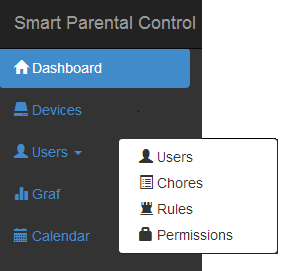
\includegraphics[width=0.50\textwidth]{images/navigationOfWebsite.png}
	\caption{Website Navigation}
	\label{fig:navigationOfWebsite}
\end{figure}


The system was also designed such that no other menu or functionality is any more than 2 clicks away, every add or detail function can be accessed directly from one of the head menus.\\

\subsection{Color Scheme and Layout Design}
%Color Schemes
%Bootstrap and other inspiration sources
The color scheme and layout design was inspired by both bootstrap and a website which utilizes bootstrap, called SB Admin\citep{sbadmin}. A standard bootstrap color scheme have been used, with a little blue added in, because of the need to keep the colors simple but no further thought was put into it.\\
The most of the design is based on standard tools from bootstrap. With exception of the table sorter functionality. Which is a JQuery tool that allows for sorting of tables.\\
Bootstrap has been chosen since it gives an okay design and it is easy to implement prototypes in bootstrap.	


\section{Implementation}
The previous section explained what each page should do, and in some detail how from the users viewpoint.

The implementation itself of the web-pages is not very interesting since they are based on a simple format of inputting the required information and submitting it to the server.\\
A few of the functionalists are however a bit more advanced. Two of these are toggling activity of a user and the page for users.\\

\subsection{Toggling Activity}
%AJAX
%PHP

Under the page Devices, the overview of tags and controllers can be seen. But this is also were the activity of a user can be toggled.

\begin{figure}[htbp]
	\centering
		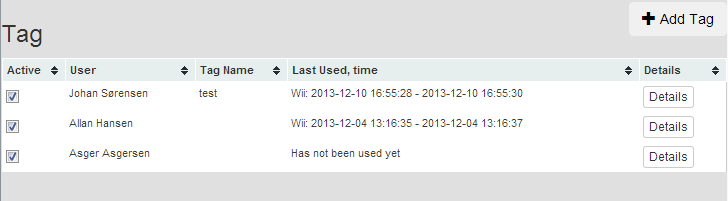
\includegraphics[width=1.00\textwidth]{images/tagOverview.PNG}
	\caption{Tag Overview}
	\label{fig:tagOverview}
\end{figure}

This is done by pressing the checkbox in the left side of the tags overview, see figure \ref{fig:tagOverview}. When this is pressed it activates an AJAX call that makes a http request to the PHP page \texttt{setActiveTag.php}. That PHP page then makes a query to the database in order to set the \texttt{active} status of a tag in the system, see figure \ref{fig:flowChartTagActivity}. Resulting in the user no longer being able to use said tag. If it is pressed again the opposite happens and the user can again use said tag.


\begin{figure}[htbp]
	\centering
		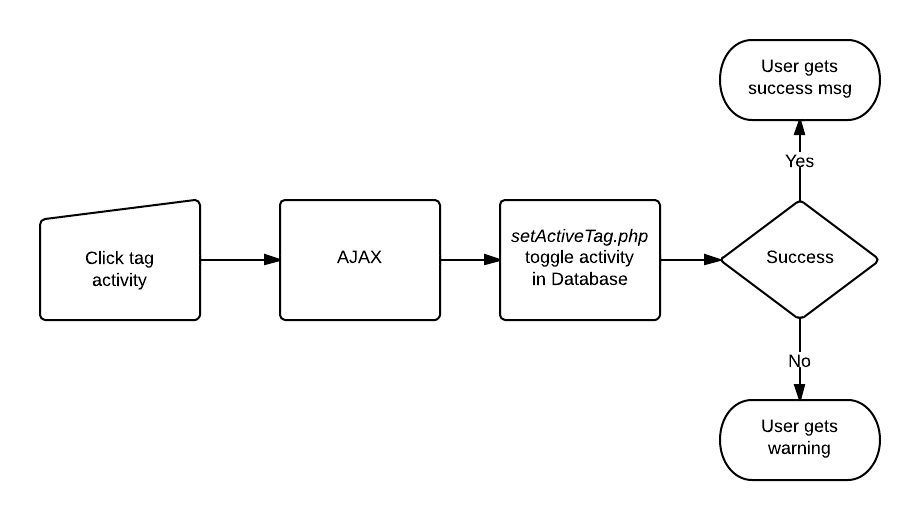
\includegraphics[width=0.75\textwidth]{images/flowChartTagActivity.png}
	\caption{Flowchart for Toggling Activity}
	\label{fig:flowChartTagActivity}
\end{figure}


\subsection{The Rules Page}
\label{subsec:rulesWEB}
The most advanced feature of the web interface is the rule page, therefor it is explained here.

\begin{figure}[htbp]
	\centering
		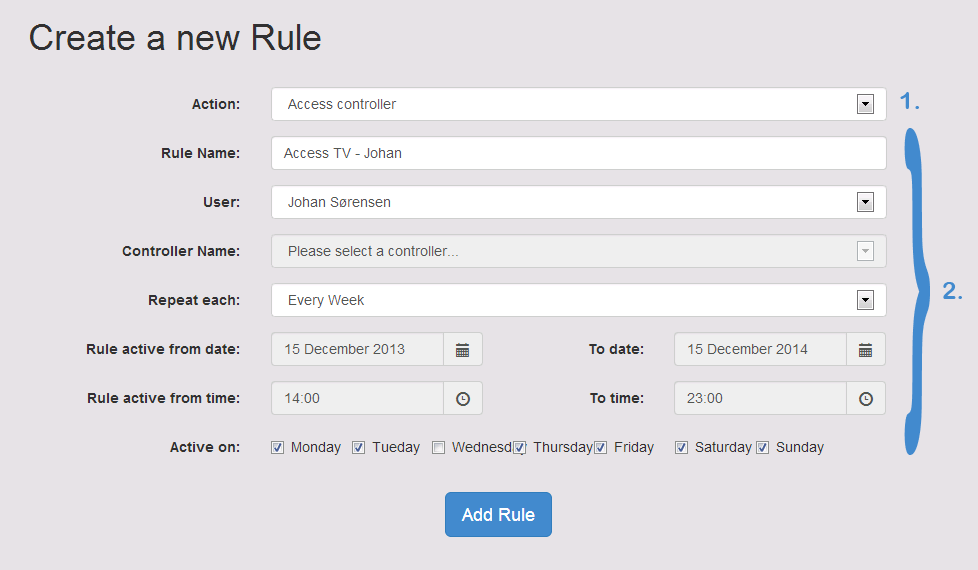
\includegraphics[width=1.00\textwidth]{images/createNewRule.png}
	\caption{Create New Rule}
	\label{fig:createNewRule}
\end{figure}

As mentioned in the Database chapter, see \vref{chap:database}, rules underwent some changes during development of the MOM system. In the design of rule it was decided that a rule could have several actions and conditions (1:many relationship), but during the development of the web page it was found that it would be too advanced for the user. Therefore it was decided that in the website a rule can have only one condition and action (1:1 relationship).\\%\fixme{lisbeth: dette er min version, jeg synes det er bere}\\ 
%As mentioned in the Database chapter, see \vref{chap:database}, rules underwent some changes during development of the MOM system. The first layout was the development teams understanding and ideas about the concept, but as the web page was created it became apparent that the first layout was too advanced, with that reasoning the rule concept went from a one:to:many concept to a one:to:one concept.\\
But that is not the only change made. The first layout was created with names for rules that fit into a computer science way of thinking. Names such as: \texttt{permissionNone}, \texttt{permissionAll}, \texttt{true} and so forth. These names have been rethought into \texttt{Cannot access any controller}, \texttt{Can access any controller} and \texttt{Unlimted points}, to fit into a pure English language.\\
Yet another change was that rules could not be set to start or end at a given time, they would simply be active constantly after creation and follow the conditional pattern give by the creator.\\
In the final version a rule no longer consists of an action and a condition, at least not from the users viewpoint. Instead they choose an action, see \ref{fig:createNewRule} mark 1., and give that action a time constraint, see \ref{fig:createNewRule} mark 2..\\
This means that conditions such as \texttt{Controller On} and \texttt{Controller Off} is now incorporated into special action names.
This is done in order to reduce the amounts of steps in a rule and also to reduce the number of decisions for a user to take during rule creation.

\subsubsection{How it works}
The changes to rules have been made clear and next is an explanation of how the page is used.\\

The flow can be seen in figure \ref{fig:CreateRuleFlowchart}. First the user selects an action, then by use of JQuery the user is meet with the right information boxes. They are hidden until they need to be filled out, this helps the user stay focused on the right info and also does not distract the user with information that is not needed.\\
\\
Next the user gives the rule a name, the name is only used in order for the user to recognize the rule at a later point, if it needs editing or removal.\\
Next the user should select the user and/or controller for the rule to affect. Whether the user has to select a user and/or controller is decided by the action they first choose.\\
Next the repeat pattern is selected. The repeat pattern changes the time constraint information boxes, such that it is possible for a user to create rules that only last for a single period of time, different sets of repeating periods of time or if the rule is to be always evaluated to true.\\

\begin{figure}[htbp]
	\centering
		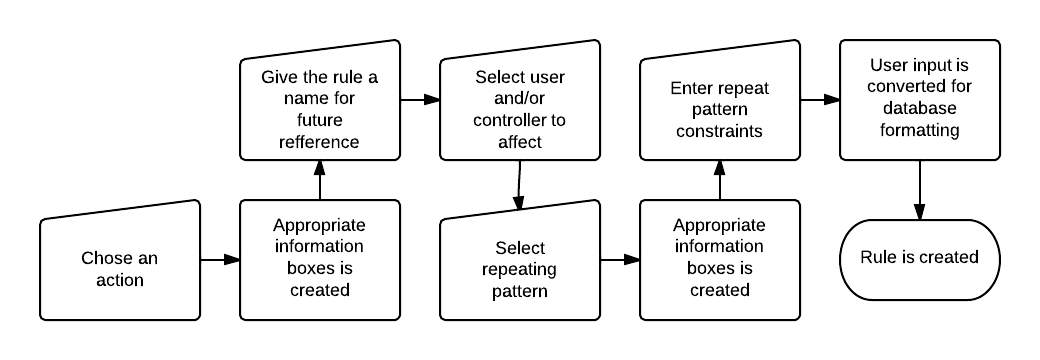
\includegraphics[width=1.50\textwidth, angle=90]{images/CreateRuleFlowchart.png}
	\caption{Create Rule Flowchart}
	\label{fig:CreateRuleFlowchart}
\end{figure}

Lastly the user enters the time constraint corresponding to the select repeat pattern, this is done by the use of graphical selectors, such that the user does not enter a wrong format of day, month, year, hour and minute.\\
When the user then submits the rule, it is formatted to fit the database. 
	\chapter{MOM Implementation}

In the previous chapters we looked at the design and implementation of the different system part there are in the Media-Online Management (MOM).
In this chapter we are going to show how it all  
	
	\chapter{Testing of the Media-Online Management}
There are different ways to evaluate the web interface e.g. an expert or user-based evaluation could be made. We would have preferred to make a user-based evaluation because this give a valuable input from a person who might use the system. However, to make such a sufficient user evaluation then we should find at least people with children which is between 5-14 years old and that would take too much time. A user-based evaluation of the entire MOM system would be optimal if the user and his/hers family could try it for a week or two before we interview them about the system. Also a log for our benefit could be made during this time to see how they use it of course with the test persons permission. Therefore to only evaluate the web interface we use an expert evaluation called Heuristic evaluation. 

\section{Heuristic evaluation in Theory}
In a Heuristic evaluation the test person(s) look for errors and potential usability errors which can be categorized in 12 item and divided into 3 groups\citep{DIEB}, which is shortly described below:
\begin{description}
\item[Learnability] make it ease for the user to learn and remembering the system:
\begin{itemize}
	\item Visibility - make it clear for the user which functions are available in the system and show what the system is doing.
	\item Consistency - be consistent in the design features and let it be similar to other comparable systems %similar systems/håber mening statid er der
	\item Familiarity - the language and symbols in the system should be familiar to the user.
	\item Affordance - let objects that look like something be it. E.g. if it looks like a button, it is a button. %pleas find en bedre sætning end 
	\fixme{'let objects that look like something be it' bedre forslag???}
\end{itemize}

\item[Effectiveness] is who ease it is for the user to use it and how safe it is to use:
\begin{itemize}
	\item Navigation - provide support to enable people to move around. Make clear navigation instructions.
	\item Control - make it clear who and what is in control, the user should be able to take control. There should be a connection between what happens in the system and what will happen outside of the system. 
	%is the mapping between control and effect. Relation what happens in system what happens in real life.
	\item Feedback - give feedback on what have happened after user do an action in the system.
	\item Recovery - how good it is to recover if the user makes an error. %e.g. user delete profile recover=> no
	\item Constraints - prevent people from doing inappropriate things in the system. This should be able to prevent serious error.
\end{itemize}

\item[Accommodation] accommodating differences between and respecting those differences:
\begin{itemize}
	\item Flexibility - let there be multiple ways of doing things.%=> dash bord if it worked
	\item Style - is the design attractive to the user. %who do it looks - attractive stylish???
	\item Conviviality - be polite and friendly. Do not use aggressive language.
\end{itemize}
\end{description}

Typically the test is done by 1-3 test persons\citep{HeuristicEvaluation}. The test person should be a usability experts or a software developer with the expertise in a relevant system. To make the test they should have relevant information of the user and a set of task to follow but they are also allowed to make their own.


\section{Heuristic Evaluation of Media-Online Management}
Before performing a Heuristic evaluation we need to determine what is needed before the evaluation is done and how the results should be presented.

\subsection{Planning the Evaluation}
When planing the evaluation the test persons need to get test persons. They need to get a small description of the user and some test cases. They should also get a list of the heuristics from which the system need to be evaluated from. This should all be made prior to the evaluation. \\

The evaluation of Media-online Management system is being done by test persons in the group which have been highly involved in the development of system. This is not optimal in this test where the test persons should be an usability expert from outside the development group.\\

The test persons also need to know the user. So the test persons need a general description of the user and their technology capabilities. The user of MOM is parents and children. The children is only in contact with the controller and the parents are both using the controller and the website. The parents has a general experience with the internet, but they are not experts. However we expect them to be able to at least set up an e-mail account with Google or Hotmail. The children has few technology skill but they are capable to turn on a normal television. \\

Before the test is conducted some test cases should be made the development team. This should cover several cases in the system such that the test persons is presented to every aspect of the system. The test cases of MOM can be found in section \vref{sec:testcase} 


(- choose the Heuristics which it should be evaluated against,(Visibility, Consistency, Control, Feedback, Familiarity is lisbeths suggestion) ) \fixme{TODO }


\subsection{Presenting the Results}
\fixme{to do}

%testcases
\section{Testcases}
\label{sec:testcase}
In table \ref{tab:testcase} is one of the test cases that we made for testing the entire Media-Online Management. In the test case both apart of the Website and a controller are tested. The change been done in the web site should affect the controller.\\ 
 All test cases can be found in appendix \vref{appen:testSuite}.
%%Test 9.
\begin{table}[h]
\label{tab:testcase}
\caption{Example of a test cases}
	\centering
		\begin{tabular*}{\textwidth}{|l|l|}
		\hline
		\hline
		Name: & \parbox{0.6\textwidth}{WS001}\\
		\hline
		Description: & \parbox{0.70\textwidth}{Setup a complete system with a managing user, a regular user,  a `TV Controller' and the accompanying rights to use it.}\\
		\hline
		Requirements: & \parbox{0.70\textwidth}{
		\begin{itemize}
			\item A computer with Internet access.
			\item The MOM website.
			\item Two Tags prepared with a Tag ID.
			\item An Arduino to function as the TV controller. 
		\end{itemize}}
		\\
		\hline
		Expected Results: & \parbox{0.70\textwidth}{A managing user capable of logging into the TV Controller without loosing points. A regular User able to log into the TV controller while loosing points.}\\
		\hline
		Steps: & \parbox{0.70\textwidth}{
		\begin{enumerate}
			\item Log into the MOM website.
			\item Create a profile with appropriate personal information to act as a manager.
			\item Attach the first Tag to the new Manager profile.
			\item Add the permissions that enables the use of all devices without expending points.
			\item Create a profile with the appropriate person information to act as a user.
			\item Attach the second tag to the new user profile.
			\item Add the permissions to log into the TV controller.
			\item Perform Test AT001A on both profiles with addendum: Wait 3 minutes for both users and note if either expends points.
		\end{enumerate}}
		\\		
		\hline
		Result of Test: & \\
		\hline
		\end{tabular*}
\end{table}


\section{Collected Results of the Heuristic Evaluation}

	%Part Perspective
	
	\part{Perspective}
	\chapter{Conclusion}
The system implementation have been explained and tested, this chapter concludes on the final product of this report.

First we need to take a look at the problem statement again.
\begin{verse}
\textit{Parents are not able to help their children administer their IT/TV consumption.\\
This results in their children getting a lessened learning ability, a bad sleeping pattern and a higher risk of type 2 diabetes.\\
How can hardware identification and webservices give parents the tools to help their children manage their media consumption?}\\
To address this problem, we face the following technical challenges:
	\begin{itemize}
		\item How do we identify unique users in a subtle and child friendly way.
		\item How do we enforce restrictions on media devices.
		\item How do we facilitate concepts as rules, permissions and chores without parents interaction.
	\end{itemize}
\end{verse}

As a whole the project gives a suggestion that is ready, with some minor updates, to be tested in a real life scenario. But the product of this project is not ready to be fully implemented in daily use or commercialized yet.\\
Before this can happen, the controller must be constructed into a state that corresponds to the specifications discussed in chapter \vref{chap:controller} and the bugs/errors found during testing must be fixed.\\
\\
However we can conclude on the technical challenges:

\section*{How do we identify unique users in a subtle and child friendly way}
%A user is identified by a tag. 
As explained in chapter \vref{chap:hardware}, we wanted to use NFC tags to identify users. However we ended up implementing this prototype with RFID, a similar technology.\\
We think that this is a concept children will be able to identify with and understand that their tag is to be used as a sort of key for the television, console or what other media connected to the controller. However this is unproven and should therefor be tested, we were not able to find any studies that show children (age 4-6) can understand and use NFC or RFID tags.\\
But in contrast to the children having to type in a password through some obscure touch- or key-interface, we think that tags are a solid implementation.

\section*{How do we facilitate concepts as rules, permissions and chores without parents interaction}
%The parent interaction has been limited to only the adding, editing and deleting of rules and permission on the website. They do not have to keep count on the time their children have been using electronic medias, since this is automatically calculated. The rules and permission is enforced by the controller. 
As explained in the Solution part  isa website created to give the parents an interface to construct rules and permissions as well as keep an overview of their children's media consumption. This takes a step forward from what parental control technologies have been available before this project. With this website we try to centralize all parental control as well as strive for making it fully automatic, meaning the parents will not have to be involved after the setup is complete.\\
The automation comes in the form of the controller, see chapter \vref{chap:controller}, being able to contact the server and confirm through the API, see chapter \vref{chap:api}, that the user (child) has access to this media and points enough to spend time on it.\\
The automation also comes in the form of the daemon, see chapter \vref{chap:daemon}, which in the current implementation makes sure the users of the system is rewarded their weekly amount of points.\\
\\
The chores, however, still require that the parents know that the child has done a chore and then manually give points to this child's profile, via the web interface. There might be a way to improve upon this, which will be discussed in the next chapter.\\
\\
This means that we have made it possible for rules and permissions to be facilitated without further parent interaction, after the setup. Which means we have succeeded in 2/3 of this challenge.
%rules and permission, website, daemon.

\section*{How do we enforce restrictions on media devices}
As explained above, we have implemented a solution that after setup results in a close to fully automatic parental control system. We have created a controller that with the help of predefined rules from the parents and an API, can restrict the usage of media devices. However during development we have not used a relay connected to the Arduino. \\
But instead we used a single LED, the code however does not need any changes for this to be used in the full scenario of the controller (Arduino and RFID reader) controlling a real TV. It is only a matter of changing the hardware connected to the pin on the Arduino.\\
\\
Therefore we say that this challenge have been completed.

\section*{Concluding on Test}
	\chapter{Future Work}
In this chapter we discuss some improvement that could be made to the Media-Online Management system.\\

\textbf{Rules}\\
The rules have been changed during the implementation. Now the web site can only add one rule to one profile, but it should be possible to add a rule or permission to several profiles. On the website a rule can only have one condition and action it would be nice if a web interface at least could support several conditions. Such that a rule like the following to be created: Peter may not watch television from 8:00 to 14:00 and 19:00 to 23:59. However if this change should not happen then the functions working with rules can be simplified. \\

\textbf{Chores}\\
It would be nice if the points for doing a chore would be more automatized such that the parents should be less involved. This could be done by a special device where the child could choose a chore and scan his tag, which then register the chore has been made. However, a parent should still approve that the chore has been done by the profile such that the child do not misuse this.\\

\textbf{Learn habits}\\
It would be nice to implement a learning algorithm that could detect a pattern in the users behavior an example if a user regularly add points to the same user then the learning algorithm can detect a pattern and make a rule that will do this. 

The data collected from this system could also be valuable statistics for studies with the users permission of course. So a data warehouse could be made to analysis the data. This data could also be used to marketing purposes. \\

\textbf{Setup of controller}\\
In section \vref{subsec:senarioD} we discussed how the system should be setup. The controller's internet connection is currently a wired connection. To make it more user friendly the controller should have WiFi connection. Then the setup of a controller will be more difficult because it is done manually. However this should be automatized such that it would be more user friendly. It could be that the user has a USB connector which can setup the wireless internet connection and add the controller to the database. 

Another possible improvement of the controller would be a wireless connection between the tag reader and the power controller device. Such that the user can scan his tag from the couch. This require some other hardware than what we had access to.\\

\textbf{Error handling}\\
The error handling for when connection between the controller and server is lost has not been fully design and implemented.  --More someone--\\

\textbf{Calendar}\\
Implement the calendar functionality fully. Where all the time bound rules are presented and the user should be able to make a rule in the calendar. It should be possible to show a calendar for one, some or all users. Other possible functionality could be import and export this calendar.\\

\textbf{Mobile application}\\
Another improvement of MOM could be to make a mobile application.\\

\textbf{The Daemon}
The daemon should detect when a controller has not contacted the service in a while and do some disciplinary actions against the user. There could also be more real time rules added which would need to be implemented in the daemon. Also other real time things such as daily/weekly reports sent via email or SMS could be implemented to give parents automatic statistics about their childs media usage. 
	
	\bibliographystyle{plain}
	\bibliography{kilder}
	\addcontentsline{toc}{chapter}{Bibliography}
	%\newpage
	\appendix
	%	\addtocounter{page}{-1}	%S�tter pagecounter til at passe med det reelle sidetal!
	%\newpage
%\addtocounter{page}{1}
\thispagestyle{empty}
\mbox{}
	
	\part{Appendix}
	\begin{appendices}
	\chapter{Rules first design}
\label{appendixFirstRuleDesign}
Before the final design had been made we used the design in this chapter.

To see a quick overview of the different conditions and their name:
\begin{description}
	\item[Timeperiode] the action can be done in this time period. 
	\item[Timestamp] the action may only happen at a given point in time. 
	\item[Controller on] the action can be done if a specific controller is turn on. 
	\item[Controller off] the action can be done if a specific controller is turn off. 
	\item[True] The action can always be taken.
\end{description}

An overview of the actions and their name is listed below:

\begin{description}
	\item[Block user] it will block the profiles of all profiles connected to the rule.
	\item[Activate user] it will activate the profiles connected to it. 
	\item[Add points] it will add points to the profiles' points.
	\item[Delete points]  it will delete points to the profiles' points.  
	\item[Set maximum of point] it will set a maximum number of points that a profile can have. 
	\item[Unlimited time] it will give the profile unlimited time to be spend on any media. 
	\item[Access any controller] it will give the profile access to any media in the system. 
	\item[Cannot access any controller] the profile will not have access to any media. 
	\item[Access controller] it will give the profile access to a specific media. 
	\item[Cannot access controller] it will block the user from using a specific media. 
\end{description}

The rule's structure is presented in a grammar in listing	\ref{grammar} expressed in Extended Backus-Naur Form(EBNF) \citep{CoPL}.
In a nonterminal is en-captured in $<>$ and a terminal is just a word or en-captured in ``''. 
Also the grouping is used represented in $()$, the replica symbol is $*$, comments is $(**)$ and alternative is $|$. 

A rule consist of a name and one of five action and condition sets which determine which actions and conditions can be combined. A rule can have several actions and conditions but only from the same set, see line 1-7. The action set is presented from 9-23 where all has a specific name, some have a specific Controller represented as a number and some has points which is a number. The condition set likewise represented from 9-23 and the condition types are presented from 25-30. There are four types but they each have a specific name. One type has Timestamp, another a Controller, the third only the name and the last is a timeperiod. The timeperiod has with two timestamp and if it is repeatable it has a string representation of the weekdays and a representation of then it is repeatable. 
\begin{lstlisting}[frame=single, label=grammar, caption=Grammar of a rule in EBNF]
<Rule>:= <name> (
	 	  (<ActionsetSet1><ConditionSet1>)*
		| (<ActionsetSet2><ConditionSet2>)*
		| (<ActionsetSet3><ConditionSet3>)*
		| (<ActionsetSet4><ConditionSet4>)*
		| (<ActionsetSet5><ConditionSet5>)*
	)

<ActionsetSet1> := "Block user" | "Activate user" 
<ConditionSet1> := <ConditionTimestamp>

<ActionsetSet2> := ("Add points" | "Delete points") <Points>
<ConditionSet2> := <ConditionTimeperiod> | <ConditionTimestamp>

<ActionsetSet3> := "Set maximum of point" <Points>
<ConditionSet3> := <ConditionTrue>

<ActionsetSet4> := "Unlimited time" | ("Access any controller" | "Cannot access any controller") <Controller>
<ConditionSet4> := <ConditionTimeperiod> | <ConditionTimestamp> 

<ActionsetSet5> := ("Access controller" | "Cannot access controller")<Controller>
<ConditionSet5> := <ConditionTimestamp> |	<ConditionTimeperiod> 
					| 	<ConditionTrue>	|	<ConditionElse>	
				
<ConditionTimestamp> :=  "Timestamp" <Timestamp>
<ConditionTimeperiod> :=  "TimePeriod" <Timestamp> <Timestamp> <Repeatable>					
<Repeatable> :=   <Weekdays> <Repeat> | Nill

<ConditionTrue> := "True" 
<ConditionElse>:= ("Device on" | "Device off") <Controller>
				
<Name> := ALPHA*  (* Upper and lowercase ASCII letters (A-Z,a-z) *)
<Controller> := DIGIT* (* Decimal digits (0-9) *)
<Points> := DIGIT*
<Timestamp> := 4*DIGIT,"-",2*DIGIT,"-",2*DIGIT, " ",2*DIGIT,":"2*DIGIT,":"2*DIGIT  (*YYYY-MM-DD HH:mm:ss*)
<Weekdays> := ("monday"| "tuesday"| "wednesday"| "thursday"| "friday"| "saturday"| "sunday")*
<Repeat> := "weekly" | "biweekly" | "triweekly" | "first in month" | "last in month"
\end{lstlisting}

	\chapter{Light Table}
\label{appen:lights}
\begin{table}[!h]
	\centering
		\begin{tabular}{| l | l |}
			\hline 
			\hline 
			\textbf{Description} & \textbf{Light Action}\\
			\hline
			Looking for connection to router & All lights blink \\
			\hline
			Looking for connection to internet & Constant red light \\
      \hline
			Ready for tag & Constant green light \\
			\hline
		  Decline user & Blinking red light in 3 seconds \\
			\hline
			Accept user & Blinking greenand orange light 3 seconds\\
			\hline
			User logged in with internetconnection & Constant green and orange \\
			\hline
			Accept new user with a current user & Blinking greenand orange light 3 seconds\\
			\hline
			Decline new user with a current user & Blinking red light 3 seconds\\
			\hline
			Disconneted with user & Constant red and orange light\\
			\hline
		\end{tabular}
\end{table}
	\chapter{Test Suite}
\label{appen:testSuite}
This chapter contain all the testcases which has been tested in the Media-Online Management system.
%%Tests to Perform.

%testcases using the website and controller
The first cases are both using the website and the controller after that it is primarily the controller and the API which is being tested.
%%Test 9.
\begin{table}[h]
	\centering
		\begin{tabular*}{\textwidth}{|l|l|}
		\hline
		\hline
		Name: & WS001\\
		\hline
		Description: & \parbox{0.70\textwidth}{Setup a complete system with a managing user, a regular user, a `TV Controller' and the accompanying rights to use it.}\\
		\hline
		Requirements: & \parbox{0.70\textwidth}{
		\begin{itemize}
			\item A computer with Internet access.
			\item The MOM website.
			\item Two Tags prepared with a Tag ID.
			\item An Arduino to function as the TV controller. 
		\end{itemize}}
		\\
		\hline
		Expected Results: & \parbox{.70\textwidth}{Adding of a regular user,tags, a `TV Controller' and the accompanying rights to use it..}\\
		\hline
		Steps: & \parbox{.70\textwidth}{
		\begin{enumerate}
			\item Log into the MOM website with lniel10 and test.
			\item Attach the first Tag to the lniel10 profile.
			\item Add the permissions that enables the use of all media without expending points.
			\item Create a profile `Kevin' with 60 points and other appropriate person information to act as a user.
			\item Attach the second tag to Kevin.
			\item Add controller TV into the system.
			\item Add the permissions to log into the TV controller.
			\item Perform Test AT001A on both profiles with addendum: Wait 3 minutes for both users and note if either expends points.
		\end{enumerate}}
		\\		
		\hline
		Result of Test: & \parbox{.70\textwidth}{The adding of controller, tag and profile were done with ease and without error. However when trying to run it with the controller it coursed several problems due to the evaluation of rules which had been out date. This is a critical error which would prevent any real communication between the controller and API. So before continuing the test this need to be fixed. When the test was resumed it worked and the results from step 8 can be found in Test AT001A.} \\
		\hline
		\end{tabular*}
\end{table}



%%Test 10.
\begin{table}[h]
	\centering
		\begin{tabular*}{\textwidth}{|l|l|}
		\hline
		\hline
		Name: & WS002\\
		\hline
		Description: & \parbox{0.70\textwidth}{Adding a rule to block a profile from using the `TV' media.}\\
		\hline
		Requirements: & \parbox{0.70\textwidth}{
		\begin{itemize}
			\item MOM Website.
			\item TV Media.
			\item Test Profile with Tag.
			\item A controller for media `TV'.
		\end{itemize}}
		\\
		\hline
		Expected Results: & \parbox{.70\textwidth}{The user attached to the profile will be unable to log into the `TV' media in accordance to the established Rule.}\\
		\hline
		Steps: & \parbox{.70\textwidth}{
		\begin{enumerate}
			\item Log into Mom Website with `lniel10' and `test'.
			\item Add Rule to block the profile, try both with a timeperiod and true.
			\item Use the controller to test if you can activate the media.
		\end{enumerate}}
		\\		
		\hline
		Result of Test: &  \parbox{.70\textwidth}{This test failed at first when making the condition true, but it succeeded with a time period. The reason for the failure was due to some changes which happened late in the implementation in connection with the rules. It is a severe error because the user expect the user to be blocked, however the severity of the problem is lessened because of how likely users would use it or even find it. This lead to another observation as it is not clear how a rule can be made true which is a moderate error since it would be a waste of time for the user but they could find a way around it.}\\
		\hline
		\end{tabular*}
\end{table}


%%Test 11.
\begin{table}[h]
	\centering
		\begin{tabular*}{\textwidth}{|l|l|}
		\hline
		\hline
		Name: & WS003\\
		\hline
		Description: & \parbox{0.70\textwidth}{Adding a rule to ensure that one media is turned on in order for another to be turned on.}\\
		\hline
		Requirements: & \parbox{0.70\textwidth}{
		\begin{itemize}
			\item A computer with Internet access.
			\item The MOM website.
			\item Web Browser with links to the API to simulate `TV'.
			\item A controller for media `Playstation'.
			\item A Tag prepared with a Tag ID.
		\end{itemize}}
		\\
		\hline
		Expected Results: & \parbox{.70\textwidth}{The simulated controller 1 will have to be turned on in order to turn on the simulated controller 2.}\\
		\hline
		Steps: & \parbox{.70\textwidth}{
		\begin{enumerate}
			\item If a `TV' controller has not been established from earlier Test, create this.
			\item Create a `Playstation' controller.
			\item Establish the Rule that the `Playstation' controller cannot be turned on unless the `TV' controller is.
			\item Use the browser to call turnOn for the `TV' and turn on the `Playstation'. \footnote{The test controller have been made to the Playstation in the mean time}
			\item If the the `Playstation' did not turn on in step 4, turn on the `TV' and then try again to turn on the `Playstation'.
		\end{enumerate}}
		\\		
		\hline
		Result of Test: & \parbox{.70\textwidth}{This test was a complete failure since the rule could not be made and when trying the user gets the message `you are missing something'. This could cause much confusion for the user that would believe it was their mistake. There are no other way to make this kind of restriction so it is a severe error but the system could function without such a rule.}\\
		\hline
		\end{tabular*}
\end{table}


%testcases to test only the controller
%%Test 1
\begin{table}[h]
	\centering
		\begin{tabular*}{\textwidth}{|l|l|}
		\hline
		\hline
		Name: & AT001A\\
		\hline
		Description: & \parbox{0.70\textwidth}{Log in and out with the Arduino and a valid Tag.}\\
		\hline
		Requirements: & \parbox{0.70\textwidth}{
		\begin{itemize}
		  \item A LED light connected to the Arduino which functions as the ``media''.
			\item Tag connected to a user with enough points and permission to use the media.
			\item The Arduino running the final software version.
			\item Serial Connection to Arduino.
			\item Web Browser with link to Status API for the media being used.
		\end{itemize}}\\
		\hline
		Expected Results: & \parbox{.70\textwidth}{When the RFID antenna detects the tag, the LED light will turn on, The Serial will note that it is now running in State 1 and the web browser will report that the Status is green.
		When swiping the tag a second time, the LED light will turn off, The Serial will report that the Arduino is running at State 0 and the webbrowser will confirm that the status is RED for not running.
		After either swipe the Arduino will be ready for a new tag swipe.}\\
		\hline
		Steps: & \parbox{.70\textwidth}{
		\begin{enumerate}
			\item Turn on the Arduino. (Wait for Serial to confirm that the device is running.)
			\item Swipe tag over RFID antenna and observe if the LED turns on.
			\item On the Serial Output, note if the State changes from 0 to 1.
			\item Confirm on the web browser that the media is marked status:GREEN  running.
			\item Swipe tag over the RFID antenna again and observe if the LED turns off.
			\item On the Serial output, note if the State changes from 1 to 0.
			\item Confirm on the web browser.
		\end{enumerate}}
		\\
		\hline
		Result of Test: & see next page.\\
		\hline
		\end{tabular*}
\end{table}
		
\begin{table}[h]
	\centering
		\begin{tabular*}{\textwidth}{|l|l|}
		\hline
		\hline
		Name: & AT001A\\
		\hline
		Description: & \parbox{0.74\textwidth}{Log in and out with the Arduino and a valid Tag.}\\
		\hline
		Result of Test: & \parbox{.74\textwidth}{First Iteration: Upon the first swipe the Arduino successfully logged in and changed state to 1 as expected. Confirmation also proved that to be status:GREEN. However, on the second swipe the Arduino would log out, but then immediately try to log in again with a corrupted Tag ID. All further attempts to log in would likewise fail due to Tag ID corruption.
		We traced the problem of the corrupted tag ID to the lack of a null character `\textbackslash 0' in the char array that held the ID's. However the Arduino would still try to log in again, which was resolved by implementing a strcmp(newID, oldID) to evaluate if the tag was different. This error is a critical problem since it is expected of the controller that it should be able to receive multiple log-ins and log-outs during the day.\\
	Second Iteration: The Arduino performed as expected, succeeding in logging users in and out.} \\
		\hline
		\end{tabular*}
\end{table}

%%Test 2.
\begin{table}[h]
	\centering
		\begin{tabular*}{\textwidth}{|l|l|}
		\hline
		\hline
		Name: & AT001B\\
		\hline
		Description: & \parbox{0.70\textwidth}{Log in with the Arduino and a Tag that does not have the proper permissions.}\\
		\hline
		Requirements: & \parbox{0.70\textwidth}{
		\begin{itemize}
		  \item A LED light connected to the Arduino which functions as the ``media''.
			\item Tag connected to a user without the permission to use the media.
			\item The Arduino running the final software version.
			\item Serial Connection To the Arduino.
			\item Web Browser with link to Status API for the media being used.
		\end{itemize}}
		\\
		\hline
		Expected Results: & \parbox{.70\textwidth}{When the RFID antenna detects the tag, the LED light will remain off, the state will remain 0 and the web browser will report that the Status is RED for not running.
		The Arduino will return to waiting for a new tag swipe.}\\
		\hline
		Steps: & \parbox{.70\textwidth}{
		\begin{enumerate}
			\item Turn on the Arduino. (Wait for Serial to confirm that the device is running.)
			\item Swipe tag over RFID antenna and observe if the LED turns on.
			\item On the Serial Output, note if the Arduino changes state.
			\item Confirm on the web browser that the media is marked status:RED for not running.
		\end{enumerate}}
		\\
		\hline
		Result of Test: & \parbox{.70\textwidth}{The Arduino performed as expected and successfully declined logging in.}\\
		\hline
		\end{tabular*}
\end{table}

%%Test 3.
\begin{table}[h]
	\centering
		\begin{tabular*}{\textwidth}{|l|l|}
		\hline
		\hline
		Name: & AT001C\\
		\hline
		Description: & \parbox{0.70\textwidth}{Log in with the Arduino and a Tag not supplied with enough points to run.}\\
		\hline
		Requirements: & \parbox{0.70\textwidth}{
		\begin{itemize}
		  \item A LED light connected to the Arduino which functions as the ``media''.
			\item Tag connected to a user without enough points to use the media.
			\item A serial connection to the Arduino
			\item The Arduino running the final software version.
			\item Web Browser with link to Status API for the media being used.
		\end{itemize}}
		\\
		\hline
		Expected Results: & \parbox{.70\textwidth}{When the RFID antenna detects the tag, the LED light will remain off, the state of the arduino will not change and the web browser will report that the Status is RED.		
		The Arduino will return to waiting for a new tag swipe.}\\
		\hline
		Steps: & \parbox{.70\textwidth}{
		\begin{enumerate}
			\item Turn on the Arduino. (Wait for Serial to confirm that the device is running.)
			\item Swipe tag over RFID antenna and observe if the LED turns on.
			\item Observe on the Serial Output if the state changes.
			\item Confirm on the web browser that the media is marked status:RED for not running.
		\end{enumerate}}
		\\
		\hline
		Result of Test: & \parbox{.70\textwidth}{The Arduino performed as expected successfully declined logging in.}\\
		\hline
		\end{tabular*}
\end{table}

%%Test 4.
\begin{table}[h]
	\centering
		\begin{tabular*}{\textwidth}{|l|l|}
		\hline
		\hline
		Name: & AT001D\\
		\hline
		Description: & \parbox{0.70\textwidth}{Log in with the Arduino and a Tag not recognized.}\\
		\hline
		Requirements: &
		\parbox{0.70\textwidth}{
		\begin{itemize}
		  \item A LED light connected to the Arduino which functions as the ``Device''.
			\item A tag that has not been introduced to the system yet.
			\item A Serial Connection to Arduino.
			\item The Arduino running the final software version.
			\item Web Browser with link to Status API for the media being used.
		\end{itemize}}\\
				\hline
		Expected Results: & \parbox{.70\textwidth}{When the RFID antenna detects the tag, the LED light will remain off, the state of the arduino will not change and the web browser will report that the Status is RED.		
		The Arduino will return to waiting for a new tag swipe.}\\
		\hline
		Steps: & \parbox{.70\textwidth}{
		\begin{enumerate}
			\item Turn on the Arduino. (Wait for Serial to confirm that the device is running.)
			\item Swipe tag over RFID antenna and observe if the LED turns on.
			\item Observe on the Serial Output if the state changes.
			\item Confirm on the web browser that the media is marked status:RED for not running.
		\end{enumerate}}
		\\
		\hline
		Result of Test: & \parbox{.70\textwidth}{The Arduino performed as expected and successfully declined logging in.}\\
		\hline
		\end{tabular*}
\end{table}

%%Test 5.
\begin{table}[h]
	\centering
		\begin{tabular*}{\textwidth}{|l|l|}
		\hline
		\hline
		Name: & AT002A\\
		\hline
		Description: & \parbox{0.70\textwidth}{Swipe a valid Tag that has the right permissions and points, while another user is logged in with the Arduino.}\\
		\hline
		Requirements: & \parbox{0.70\textwidth}{
		\begin{itemize}
		  \item A LED light connected to the Arduino which functions as the ``media''.
			\item Tag connected to a user with enough points and permission to use the media.
			\item A second Tag connected to a user with enough points and permission to use the media.
			\item The Arduino running the final software version.
			\item Web Browser with link to Status API for the media being used.
		\end{itemize}}
		\\
		\hline
		Expected Results: & \parbox{.70\textwidth}{When the second tag is swiped while the first user is still active the LED should briefly flicker off and then on again as the new user logs back in.}\\
		\hline
		Steps: & \parbox{.70\textwidth}{
		\begin{enumerate}
			\item Turn on the Arduino. (Wait for Serial to confirm that the device is running.)
			\item Swipe tag over RFID antenna and observe if the LED turns on.
			\item Confirm on the web browser that the media is marked status:GREEEN for running.
			\item Swipe tag over RFID antenna and observe if the LED Turns off and then on again.
			\item Confirm on the web browser that the media is still marked status:GREEEN for running.
		\end{enumerate}}
		\\
		\hline
		Result of Test: & \parbox{.70\textwidth}{The Arduino performed as expected and successfully logged user 1 off before logging user 2 in due to the corrections performed after Test AT001A.}\\
		\hline
		\end{tabular*}
\end{table}
%%Test 6.
\begin{table}[h]
	\centering
		\begin{tabular*}{\textwidth}{|l|l|}
		\hline
		\hline
		Name: & AT003A\\
		\hline
		Description: & \parbox{0.70\textwidth}{Let Arduino run until getStatus is called without logged in User.}\\
		\hline
		Requirements: & \parbox{0.70\textwidth}{
		\begin{itemize}
			\item The Arduino running the final software version.
			\item Web Browser with link to Status API for the media being used.
			\item Serial Connection to Arduino.
		\end{itemize}}
		\\
		\hline
		Expected Results: & \parbox{.70\textwidth}{Run smoothly, remain in State 0, Remain turned off.}\\
		\hline
		Steps: & \parbox{.70\textwidth}{
		\begin{enumerate}
			\item Turn on the Arduino. (Wait for Serial to confirm that the device is running.)
			\item Wait and confirm that the status has run with the Serial Watch and note if its Status:RED.
			\item Confirm on the web browser that the media is still marked status:RED for running.
		\end{enumerate}}
		\\
		\hline
		Result of Test: & \parbox{.70\textwidth}{Initially we believed there was a bug where the Arduino would freeze after the getStatus being called the second time, but we have not since been able to reproduce it and after seeing the Arduino run unhindered for hours at the time we conclude that it is running as expected.}\\
		\hline
		\end{tabular*}
\end{table}

%%Test 7.
\begin{table}[h]
	\centering
		\begin{tabular*}{\textwidth}{|l|l|}
		\hline
		\hline
		Name: & AT003B\\
		\hline
		Description: & \parbox{0.70\textwidth}{Let Arduino run until getStatus is called with logged in User.}\\
		\hline
		Requirements: & \parbox{0.70\textwidth}{
		\begin{itemize}
			\item The Arduino running the final software version.
			\item Tag connected to a user with enough points and permission to use the media.
			\item A serial connection to the Arduino.
			\item Web Browser with link to Status API for the media being used.
		\end{itemize}}\\
		\hline
		Expected Results: & \parbox{.70\textwidth}{The User will Remain logged in and the Arduino will not change from state 1.}
		\\
		\hline
		Steps: & \parbox{.70\textwidth}{
		\begin{enumerate}
			\item Turn on the Arduino. (Wait for Serial to confirm that the device is running.)
			\item Swipe tag over RFID antenna and observe if the LED turns on.
			\item Wait and confirm that the status has run with the Serial Watch and note if its Status:GREEN.
			\item Note if the Arduino changes state.
			\item Confirm that the LED remains on.
			\item Confirm on the web browser that the media is still marked status:GREEN for running.
		\end{enumerate}}
		\\
		\hline
		Result of Test: & \parbox{.70\textwidth}{The Arduino performed as expected and remained logged in after the getStatus had been called.}\\
		\hline
		\end{tabular*}
\end{table}

%%Test 8.
\begin{table}[h]
	\centering
		\begin{tabular*}{\textwidth}{|l|l|}
		\hline
		\hline
		Name: & AT003C\\
		\hline
		Description: & \parbox{0.70\textwidth}{Let Arduino run until getStatus is called with logged in User, who has since logging in have his rights to use the media revoked.}\\
		\hline
		Requirements: & \parbox{0.70\textwidth}{
		\begin{itemize}
			\item The Arduino running the final software version.
			\item Tag connected to a user with enough points and permission to use the media.
			\item Access to the website MOM
			\item A serial connection to the Arduino.
			\item Web Browser with link to Status API for the media being used.
		\end{itemize}}
		\\
		\hline
		Expected Results: & \parbox{.70\textwidth}{The Arduino will run with user logged in, state 1, and with the LED turned on until the timer is reached. 
		Then the user will be logged out, the LED will turn off and the Arduino will move to state 0.}\\
		\hline
		Steps: & \parbox{.70\textwidth}{
		\begin{enumerate}
			\item Turn on the Arduino. (Wait for Serial to confirm that the device is running.)
			\item Swipe tag  over RFID antenna and observe if the LED turns on.
			\item Confirm on the web browser that the media is still marked status:GREEN for running.
			\item Use the Web Site to revoke permission to the media.
			\item Use browser to confirm that the media is marked as status:RED.
			\item Wait and confirm that the status has run with the Serial Watch and note if its Status:RED.
			\item Confirm that the LED turns off.
		\end{enumerate}}
		\\		
		\hline
		Result of Test: & \parbox{.70\textwidth}{First Iteration: It turned out that the API did not actually support any aspect of this feature. The error was if a permission granted the access then it was not checked whether he still had that permission. It is a moderate error since this can only happen once per permission lifetime. This has since been rectified. \\Second Iteration: The Arduino now performs as expected.}\\
		\hline
		\end{tabular*}
\end{table}


	\end{appendices}
	
	%Denne komando lister alle fixme's
	%\part{Fixme}
	%\listoffixmes

\end{document}
